\documentclass{scrartcl}

\usepackage[utf8]{inputenc}
\usepackage{hyperref}
\usepackage{url}
\usepackage{graphicx}
\usepackage{amssymb}
\usepackage[T1]{fontenc}
\usepackage{blkarray}
\usepackage{caption}
\usepackage{subcaption}
\usepackage{biblatex}
\usepackage{amsmath}
% \usemintedstyle{vs}
\usepackage{svg}
\usepackage[many]{tcolorbox}    	% for COLORED BOXES (tikz and xcolor included)
\addbibresource{bibliography.bib} 
\newtcolorbox{boxK}{
    sharpish corners, % better drop shadow
    boxrule = 0pt,
    toprule = 4.5pt, % top rule weight
    enhanced,
    fuzzy shadow = {0pt}{-2pt}{-0.5pt}{0.5pt}{black!35} % {xshift}{yshift}{offset}{step}{options} 
}

\newcommand{\emailaddr}[1]{\href{mailto:#1}{\texttt{#1}}}


\title{Cleaning Agents with DeepQLearning
\\
A perfomance comparison betwen MLP and RNN networks
\\
\begin{small} 
  Final report for the course of Intelligent Systems Engineering  - 
  MS Engineering and Computer Science
\end{small}
}
\author{
    \emailaddr{filippo.cavallari2@studio.unibo.it}
}
\date{\today}

\begin{document}

\maketitle

\newpage

\begin{abstract}
  In this report, I investigate the application of Deep Reinforcement Learning (DRL) techniques, tailored for 
  Multilayer Perceptron (MLP) and Long Short-Term Memory Recurrent Neural Networks (LSTM RNN), within VMAS 
  (Vectorized Multi-Agent Simulator).
  My study introduces the "Cleaning Agents" scenario, where N agents are tasked with efficiently cleaning M 
  stationary targets in a 2D space. The central goal of this project is to evaluate and compare the impact of 
  DRL methods, specifically MLP and LSTM RNN, on agent coordination and decision-making within this scenario.
  
  To achieve this goal, I employ time-based performance metrics to assess the efficiency and effectiveness of 
  these DRL variants. By quantifying the temporal aspects of agent behavior, I aim to provide practical insights 
  into the application of DRL in multi-agent systems. This comparative analysis offers valuable guidance for selecting the 
  most suitable DRL architecture for similar multi-agent tasks.\end{abstract}
\newpage
\tableofcontents

\newpage
\listoffigures

\newpage

\section{MARL}

\subsection{Overview}
A multi-agent system comprises multiple entities that, with a certain degree of independence, make decisions 
and interact with each other within an environment \cite{weiss1999multiagent}. Each agent is assigned a task to pursue, which can be 
either the same as others (cooperative) or different (competitive). To address a specific task, an agent 
requires a set of skills. Expressing these competencies programmatically would be particularly complex. Hence, the decision was made to employ Reinforcement Learning, 
giving rise to the term Multi-Agent 
Reinforcement Learning, for which the following definition can be provided:

"A group of agents collectively learns the best policy to maximize a long-term reward function."

\subsection{Environment}
These two characteristics introduce complexities compared to Single-Agent Reinforcement 
Learning (SARL). In SARL, the learning process is modeled as a Markov Decision Process (MDP),
 which is inherently stationary by definition. Consequently, SARL inherently assumes a single
  agent engaged in the learning process, with the remaining agents considered as part of the 
  environment.

In the case of MARL, Reinforcement Learning is integrated using an additional abstraction 
known as Stochastic Game S (or Markov Games) \cite{LITTMAN1994157}:

\begin{itemize}
  \item $\mathcal{S}$ is a tuple $<N, S, \{A^i\}, P,  \{R^i\}>$ with $i \in 1..N$
  \item N is the number of agents (must be greaten than 1 but has no upper-bound)
  \item S is always a space of values that represent the global state of the system
  \item $A^i$ is the action space of the i-th agent
  \begin{itemize}
       \item The global space is defined as $\mathbb{A} = A^1 \times A^2 \times .... \times A^N$
  \end{itemize}
  \item $P: S \times \mathbb{A} \rightarrow \mathcal{P}(S)$ is the function that describes the steps between each state
  \begin{itemize}
      \item $P(S)$ is discrete probability distribution that pairs each state $s \in S$ with a probability
  \end{itemize}
  \item $R^i: S \times \mathbb{A} \times S \rightarrow \mathbb{R}$ is the reward function
\end{itemize}

\begin{boxK}
\textbf{\textit{Example of Markov Game: Paper, Rock and Scissor}}

  \begin{itemize}
    \item $N = 2$
    \item $A^1 = A^2 = $ \{Paper, Rock, Scissor\}
    \item $S = $ \{ \}
    \item $R = \begin{blockarray}{cccc}
      & Rock & Paper & Scissor \\
    \begin{block}{c[ccc]}
      Rock    & 0, 0  & -1, 1 & 1, -1 \\
      Paper   & 1, -1 & 0, 0  & -1, 1 \\
      Scissor & -1, 1 & 1, -1 & 0, 0 \\
    \end{block}
  \end{blockarray}$
  \end{itemize}
\end{boxK}

\subsubsection{Types of MARL}
MARL systems can be categorized in various ways, and one primary division is as follows \cite{4445757}:

% \begin{figure}
%     \centering
%     \includesvg[width=11cm]{img/MARL-Divisione1.svg}
% \end{figure}

\begin{itemize}
    \item \textbf{\textit{Cooperative}}: In cooperative MARL, all agents within the system share the same goal, and consequently, the same reward function $(R^1 = ... = R^i = ... = R^N)$.
    \begin{itemize}
        \item \textbf{\textit{Homogeneous}}: In homogeneous cooperative MARL, all agents have identical capabilities $(A^1 = ... = A^i = ... = A^N)$; the overall objective is to find the best policy. % which is usually the same for each agent $(\pi^* = \pi^*_1 = ... = \pi^*_N)$.
        \item \textbf{\textit{Heterogeneous}}: In heterogeneous cooperative MARL, agents may possess varying capabilities, and in the worst-case scenario, each agent has different capabilities from all others $(A^1 \neq ... \neq A^i \neq ... \neq A^N)$. The global objective is to maximize each agent's local policy while pursuing the shared goal.
    \end{itemize}
    \item \textbf{\textit{Competitive}}: Competitive MARL involves agents with different goals who compete to maximize their own reward functions. A typical example of such systems is board games.
    \item \textbf{\textit{Mixed}}: In mixed MARL, both cooperative agents with a shared goal and competitive agents with different goals coexist. A classic example is team-based games where players on the same team cooperate while players from different teams compete.
\end{itemize}

Further division can be made based on how the training and execution of various agents occur:

% \begin{figure}
%     \centering
%     \includesvg[width=11cm]{img/MARL-Divisione2.svg}
% \end{figure}

\begin{itemize}
    \begin{figure}
    \centering
    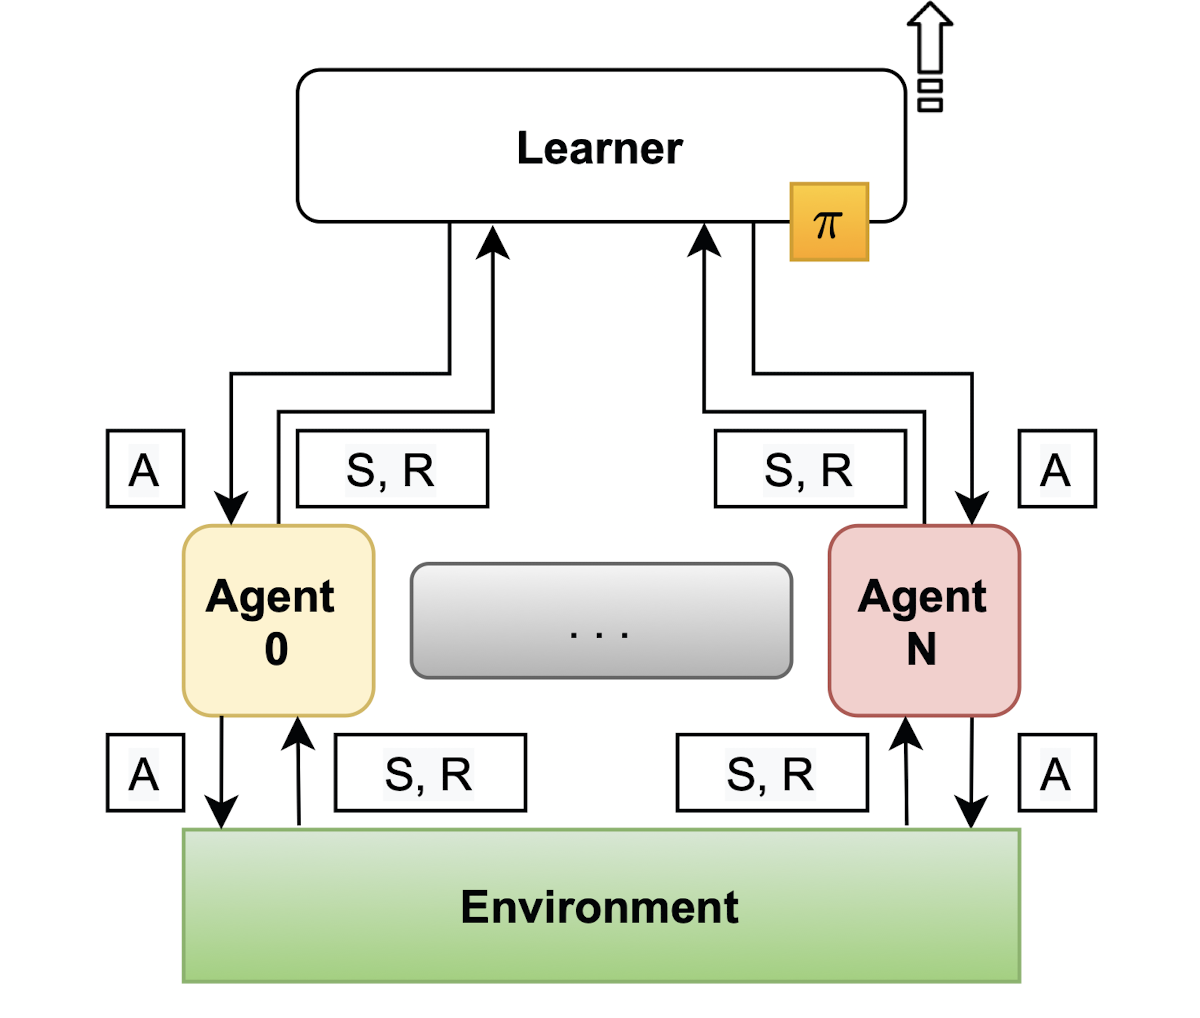
\includegraphics[width=8cm]{img/CTCE.png}
    \caption{CTCE System \cite{aguzzi}}
    \label{fig:a}
    \end{figure}

    \item \textbf{\textit{Centralized Training Centralized Execution}} [\ref{fig:a}]: In this type of system, a higher-level "Learner" agent with a global perspective is responsible for training and computing actions. The remaining agents send their local environment perceptions (local states) to the Learner agent, who reconstructs the global state. The Learner agent then selects actions according to the current policy, evaluates reward functions, and updates the policy (learning process). This approach is typically used for offline training of the system.
    
    \begin{figure}
    \centering
    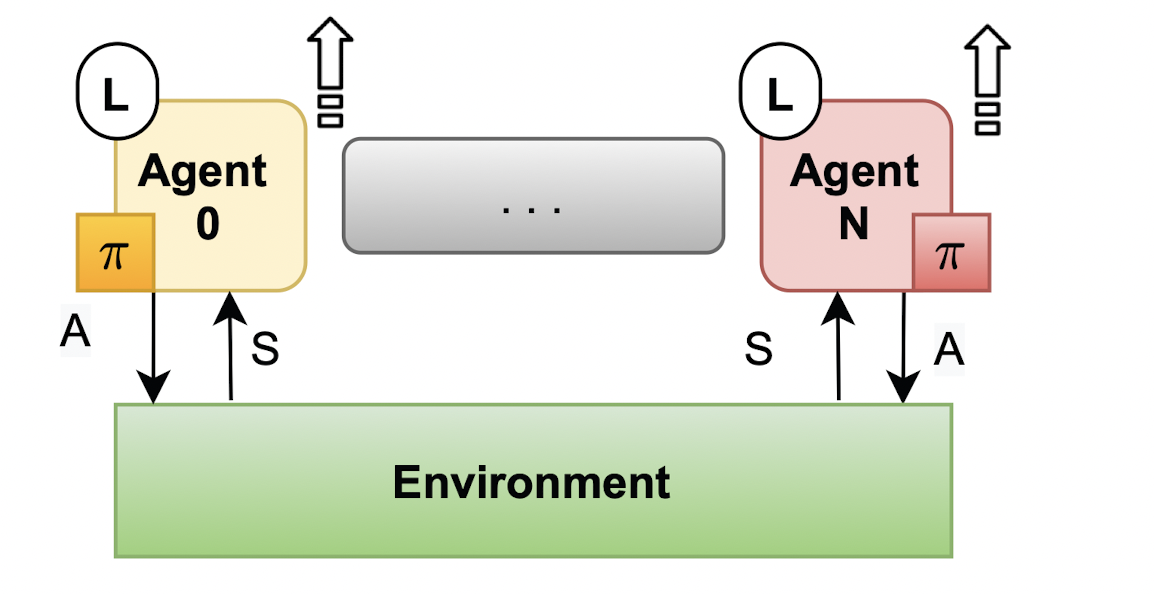
\includegraphics[width=8cm]{img/DTDE.png}
    \caption{DTDE System \cite{aguzzi}}
    \label{fig:b}
    \end{figure}

    \item \textbf{\textit{Decentralized Training Decentralized Execution}} [\ref{fig:b}]: In this type of system, each agent has its local policy and can only perceive a portion of the environment. Each agent takes actions based on its perception of the environment, updating its local reward function accordingly. This approach is used for both offline training and online deployment of the system.
    
    \begin{figure}
      \centering
      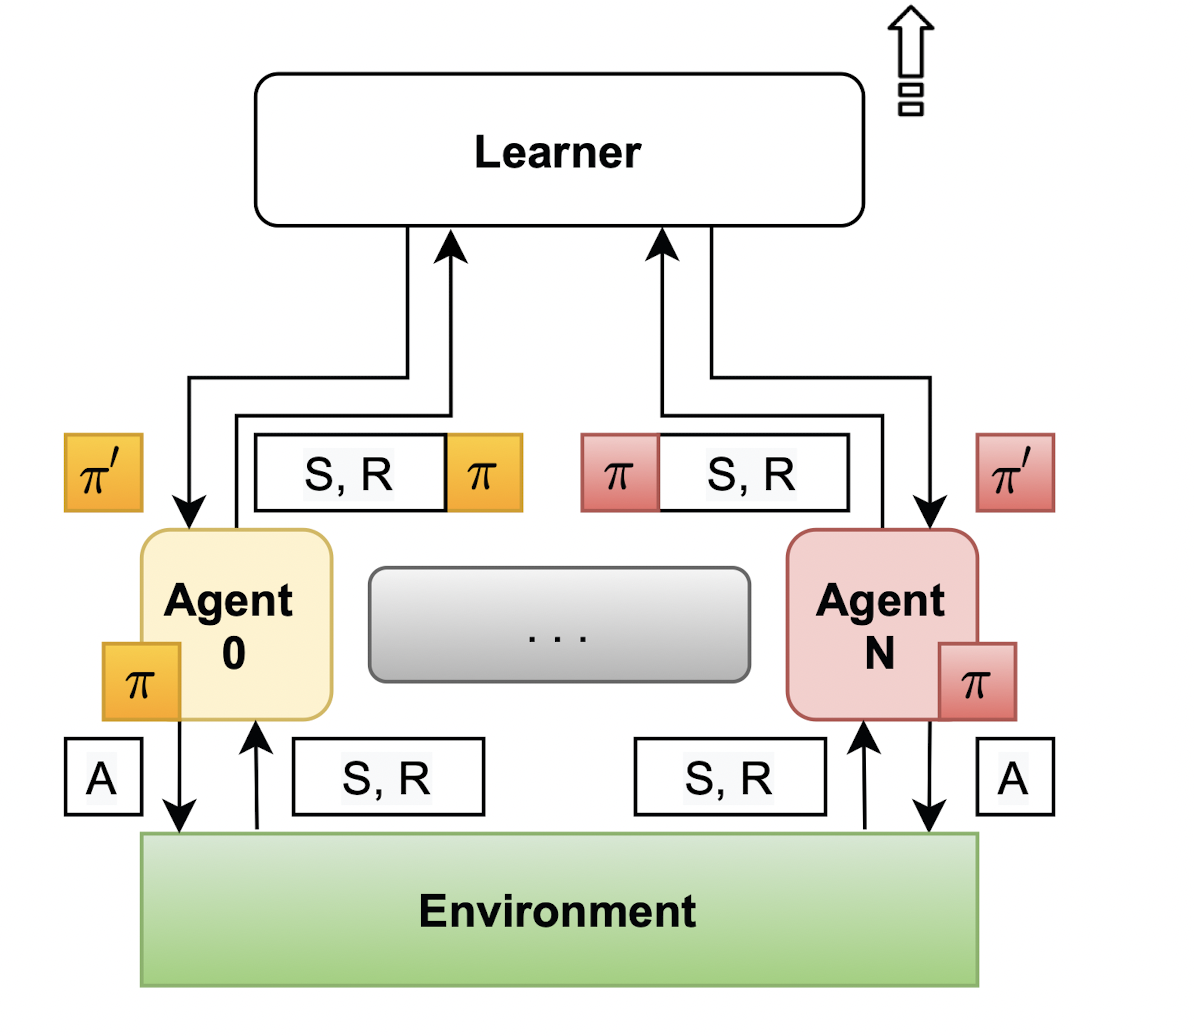
\includegraphics[width=8cm]{img/CTDE.png}
      \caption{CTDE System \cite{aguzzi}}
      \label{fig:c}
      \end{figure}
    
    \item \textbf{\textit{Centralized Training Decentralized Execution}} [\ref{fig:c}]: In this type of system, two distinct steps are involved:
    \begin{enumerate}
        \item \textbf{\textit{Simulation Time}}: Each agent uses its local policy, and at the end of each episode, they send their respective information to a central Learner agent. This Learner agent, with a global view of the environment, updates the local policies of the various agents.
        \item \textbf{\textit{Execution Time}}: During this phase, each agent uses its local policy (resulting from the training process) to interact with the environment.
    \end{enumerate}
    
\end{itemize}


\newpage

\section{Deep Q-Learning}

\subsection{Overview}

Deep Q-Learning (DQL) represents a significant advancement in the field of Reinforcement Learning (RL) by combining Q-Learning principles with deep neural networks. This chapter provides a comprehensive exploration of DQL, covering its core concepts, underlying algorithms, the Bellman equation, and practical applications \cite{DBLP:journals/corr/MnihKSGAWR13}.

\subsection{Background}

\subsubsection{Reinforcement Learning}

Reinforcement Learning is a machine learning paradigm focused on training agents to make sequences of decisions within an environment to maximize cumulative rewards. It has gained popularity in various domains, including robotics, gaming, recommendation systems, and autonomous navigation.

\subsubsection{Q-Learning}

Q-Learning is a foundational RL algorithm that learns an action-value function, denoted as $Q(s, a)$, to estimate the expected cumulative reward an agent can achieve by taking a specific action $a$ in a given state $s$ and following an optimal policy. It employs an iterative update rule to refine these Q-values until they converge to the optimal values.

\subsection{Deep Q-Learning Basics}

\subsubsection{The Q-Function}

In DQL, the Q-function is represented as a deep neural network. This network takes the current state $s$ as input and outputs a Q-value for each possible action $a$. The agent selects the action with the highest Q-value, guiding its decision-making process.

\subsubsection{Q-Loss Function}

To train the deep Q-network (DQN), a loss function is defined to measure the discrepancy between predicted Q-values and target Q-values. The loss function aims to minimize the difference between the predicted and target Q-values.

The Q-learning loss is typically calculated as follows:
\[
L(\theta) = \mathbb{E}\left[(Q(s, a;\theta) - (r + \gamma \max_{a'}Q(s', a';\theta^-))^2\right]
\]
where:
\begin{align*}
L(\theta) & \text{ is the loss with respect to the network's parameters }\theta. \\
Q(s, a;\theta) & \text{ is the predicted Q-value for state }s\text{ and action }a\text{ with network parameters }\theta. \\
r & \text{ is the immediate reward received after taking action }a\text{ in state }s. \\
\gamma & \text{ is the discount factor that determines the importance of future rewards.} \\
s' & \text{ is the next state after taking action }a\text{ in state }s. \\
\theta^- & \text{ are the parameters of the target Q-network.}
\end{align*}

\subsubsection{Experience Replay}

One of the critical components of DQL is experience replay. It involves storing a replay buffer of past experiences $(s, a, r, s')$ (state, action, reward, next state) and sampling mini-batches from it during training. Experience replay helps stabilize training and breaks the temporal correlations present in sequential data.

\subsubsection{Target Network}

To further stabilize training, DQL employs a target network, which is a copy of the Q-network with delayed updates. The target network provides a stable Q-value target for the loss calculation.

\subsubsection{Exploration vs. Exploitation}

Balancing exploration (trying new actions) and exploitation (choosing the best-known action) is essential in DQL. The $\epsilon$-greedy policy is commonly used, where the agent selects the best action with probability $(1-\epsilon)$ and explores with probability $\epsilon$.

\subsection{The Bellman Equation for Q-Value Approximation}

The Bellman equation plays a crucial role in Q-Learning and DQL. It expresses the Q-value of a state-action pair as the sum of the immediate reward and the discounted maximum Q-value of the next state-action pair:

\[
Q(s, a) = r + \gamma \max_{a'} Q(s', a')
\]

Where:
\begin{align*}
Q(s, a) & \text{ is the Q-value of state }s\text{ and action }a. \\
r & \text{ is the immediate reward for taking action }a\text{ in state }s. \\
\gamma & \text{ is the discount factor determining the importance of future rewards.} \\
s' & \text{ is the next state resulting from taking action }a\text{ in state }s. \\
\max_{a'} Q(s', a') & \text{ represents the maximum Q-value achievable in the next state }s' \\
\text{ considering all possible actions }a'.
\end{align*}

\subsection{DQL Algorithm}

The core DQL algorithm can be summarized in several steps:

\begin{enumerate}
\item Initialize Q-network and target network with random weights.
\item Initialize replay buffer.
\item For each episode:
   \begin{enumerate}
   \item Observe the current state $s$.
   \item Select an action $a$ using $\epsilon$-greedy policy.
   \item Execute action $a$, observe reward $r$ and next state $s'$.
   \item Store the experience $(s, a, r, s')$ in the replay buffer.
   \item Sample a mini-batch from the replay buffer.
   \item Calculate the target Q-values using the target network.
   \item Calculate the loss between predicted and target Q-values using the Bellman equation.
   \item Update the Q-network weights using backpropagation.
   \item Periodically update the target network weights.
   \item Repeat until convergence or a predetermined number of episodes.
   \end{enumerate}
\end{enumerate}

\subsection{Challenges and Improvements}

While DQL has achieved remarkable success, it faces challenges such as training instability, Q-value overestimation, and the need for extensive data collection. Researchers have proposed various improvements, including Double DQN, Prioritized Experience Replay, and Dueling DQN, to address these issues.

\subsection{Applications of Deep Q-Learning}

DQL has been successfully applied to a wide range of problems, including but not limited to:

\begin{enumerate}
\item \textbf{Atari Games}: DQL achieved human-level performance on various Atari 2600 games, demonstrating its capability to learn complex strategies.
\item \textbf{Robotics}: DQL has been used to train robots for tasks like object manipulation, navigation, and control.
\item \textbf{Autonomous Vehicles}: DQL is employed in training autonomous vehicles for safe and efficient navigation.
\item \textbf{Recommendation Systems}: It is utilized to optimize recommendations for users on online platforms.
\item \textbf{Healthcare}: DQL is applied for optimizing treatment plans and resource allocation in healthcare.
\end{enumerate}

\newpage

\section{Vectorized Multi-Agent Simulator (VMAS)}

\subsection{Overview}

VMAS is a sophisticated framework tailored for Multi-Agent Reinforcement Learning (MARL) applications. It offers a unique blend of features and capabilities, making it a valuable tool for researchers and practitioners in the field \cite{bettini2022vmas}.

\subsection{Overview}

VMAS seamlessly combines two key advantages: vectorization and 2D physics simulation, all implemented within the PyTorch framework. Its primary purpose is to provide a diverse set of twelve complex multi-robot scenarios, each meticulously designed to present distinct challenges to state-of-the-art MARL algorithms. What sets VMAS apart is its user-friendly and modular interface, which simplifies the creation of new scenarios, fostering community contributions and collaborative development.

\subsection{Vectorized Simulation Engine}

One of VMAS's standout features is its highly efficient vectorized simulation engine. This engine empowers parallel simulations to run effortlessly on accelerated hardware, even at an extensive scale. Unlike traditional frameworks like OpenAI Multi-Agent Particle Environment (MPE), which exhibit linear increases in execution time as the number of simulations grows, VMAS excels. It can execute an impressive 30,000 parallel simulations in under 10 seconds, marking a performance improvement of more than 100 times.

\subsection{Challenging Scenarios}

VMAS is bundled with a diverse array of scenarios, each carefully crafted to challenge MARL algorithms in various ways. These scenarios feature agents and landmarks of different shapes, support rotations, incorporate elastic collisions, utilize joints, and permit custom gravity settings. The motion models for agents within VMAS are holonomic, streamlining the simulation process. Moreover, VMAS offers support for custom sensors, including LIDARs, and facilitates inter-agent communication. This breadth of scenarios opens up opportunities for exploring a wide spectrum of multi-robot coordination tasks.

\newpage

\section{Cleaning Agents Scenario}

The "Cleaning Agents" scenario within VMAS presents a challengin MARL environment. In this scenario, a team of N agents is tasked with cleaning a 2D space by removing M stationary targets. This scenario might serve as a valuable benchmark for evaluating the coordination and decision-making capabilities of MARL algorithms.

\subsection{Agents and Sensors}

Each agent in the "Cleaning Agents" scenario is equipped with a specialized LIDAR sensor that projects 50 rays into the environment. This sensor is designed to detect only targets within its range. The purpose of the LIDAR sensor is to enable agents to perceive the presence and location of targets, crucial for their cleaning task.

\subsection{Objective}

The primary goal of the agents in this scenario is to efficiently remove all M targets from the 2D space. To successfully remove a target, an agent must be in close proximity to it, ensuring effective cleaning. This proximity requirement adds complexity to the task, as agents must navigate and coordinate to reach and clean targets efficiently.

\subsection{Reward Function}

The reward function in the "Cleaning Agents" scenario is designed to encourage agents to make optimal decisions while cleaning the targets. The reward function operates as follows:
\begin{enumerate}
  \item When an agent's distance from a target falls below a predefined threshold (K), indicating successful cleaning, the agent is rewarded positively:
  Reward = $1 + \text{number of previously removed targets}$
  \item If an agent's LIDAR sensor does not detect any targets in its vicinity, it receives a negative reward (-1):
  Reward = $-1$
  \item When an agent's LIDAR sensor detects a target, and the distance from the agent's previous position to the target decreases, the agent is rewarded based on the function:
  Reward = $\frac{-\text{LIDAR range}}{x}$ (normalized to fall within the range of -0.5 to 0)
  \item Conversely, if the distance from the agent's previous position to the target increases, indicating a suboptimal move, the agent is penalized based on the same function:
  Reward = $\frac{-\text{LIDAR range}}{x}$ (normalized to fall within the range of -1 to -0.5)
\end{enumerate}
The strategic use of negative rewards, except for successful target removal, ensures that agents are motivated to make coordinated and efficient moves. It encourages agents to continually improve their performance by minimizing suboptimal actions and maximizing successful cleaning operations.

The "Cleaning Agents" scenario in VMAS thus presents a dynamic and challenging environment that tests the coordination, navigation, and decision-making capabilities of MARL algorithms in the context of multi-agent systems.

\section{Implementation}
\subsection{Custom Implementation for LSTM RNN Networks}

In my pursuit of enhancing the capabilities of Deep Q Learning (DQL), I have developed a custom implementation tailored to 
Long Short-Term Memory Recurrent Neural Networks (LSTM RNNs). This specialized approach leverages LSTM networks to capture temporal 
dependencies and improve decision-making in dynamic environments. In this subsection, I outline the key components and strategies 
employed in my custom LSTM-based DQL implementation.

\subsubsection{Utilizing the Replay Buffer for Temporal Sequences} 

One of the fundamental challenges in employing LSTM networks is the requirement for temporally consecutive states. To address this, 
I have extended the functionality of the Replay Buffer. In my modified setup, states are no longer solely composed of LIDAR 
measurements but are now augmented with the action taken by the agent and the corresponding reward received.

To feed sequences of states into the LSTM network, I require N consecutive states. I accomplish this by selecting the N-1 states 
stored in the Replay Buffer, which were observed before the current state. The current state, however, does not yet possess an 
associated action and reward, as it awaits processing by the behavioral policy. To accommodate this, I initialize tensors of the 
appropriate shape, filled with zeros, representing no action performed and no reward received.

\subsubsection{Generating Sequences for Network Improvement}

To train the LSTM-based DQL effectively, I need to generate batches of sequences that preserve the temporal structure of the data. This ensures that the LSTM can learn and generalize from the sequential patterns in the state-action-reward sequences.

To achieve this, I employ a two-step process. First, I randomly select a BATCH SIZE number of lists of consecutive random indices from the Replay Buffer. These indices are used to retrieve the corresponding states from the Replay Buffer, forming sequences that encapsulate the temporal progression of the agent's experiences.

However, it's crucial to note that this approach necessitates populating the Replay Buffer with a substantial amount of data initially. This implies that a substantial number of steps, determined by the hyperparameter settings, must be taken before initiating the network improvement process. This initial data collection phase is essential for providing sufficient training samples that enable the LSTM network to effectively capture and learn from temporal dependencies in the agent's experiences.

In summary, my custom implementation for LSTM RNN networks extends the capabilities of traditional DQL by incorporating LSTM networks to handle temporal dependencies. This adaptation includes modifying the state representation in the Replay Buffer and introducing a strategy for generating batches of sequences for network improvement. While it requires an initial data collection phase, the result is a powerful and flexible framework for addressing complex decision-making tasks in dynamic environments.

\subsection{Deep Q Learning for MLP Networks}

My implementation of Deep Q Learning (DQL) for Multilayer Perceptron (MLP) networks is designed to accommodate the unique 
characteristics of the Vectorized Multi-Agent Simulator (VMAS) environment. VMAS employs additional dimensions to parallelize 
environments and agents, necessitating a flexible approach to handle complex tensor shapes.

\subsubsection{State Representation}

In such implementation, I employ a state representation that aligns with the structure of VMAS. Specifically, the state of each agent is represented as a tensor of shape [50, 1]. This choice is informed by the fact that each agent's LIDAR sensor in VMAS emits 50 rays, returning float distances. The positions of the individual agents within the environment are not considered relevant for decision-making since agents rely solely on LIDAR measurements, and the positions of targets can vary across different VMAS environments.

\subsubsection{Tensor Shapes}

To facilitate the training and execution of the MLP networks within VMAS, my network architecture accommodates tensors with the shape [number of environments, number of agents, 50, 1]. This tensor shape aligns with VMAS's parallelized structure, allowing the network to process data from multiple environments and agents simultaneously.

By adapting my DQL implementation to handle tensors of complex shapes, I ensure seamless integration with VMAS's multi-agent framework. This flexibility enables agents to effectively learn and make decisions within the dynamic and parallelized VMAS environment, ultimately enhancing their performance in complex multi-agent tasks.

\newpage

\section{Results}
\subsection{Performance Results: MLP Networks in the Cleaning Agents Scenario}

The performance evaluation of my Multilayer Perceptron (MLP) network-based agents in the Cleaning Agents scenario provides valuable insights into their learning and decision-making capabilities. The training process consisted of 150 epochs, each comprising 1000 steps. If an agent successfully achieved its task before completing all the steps in an epoch, it proceeded to the next epoch. Here, I present a comprehensive analysis of the training and evaluation results.

\subsubsection{Training Progress}

\begin{figure}
  \centering
  \begin{subfigure}[b]{0.45\textwidth}
      \centering
      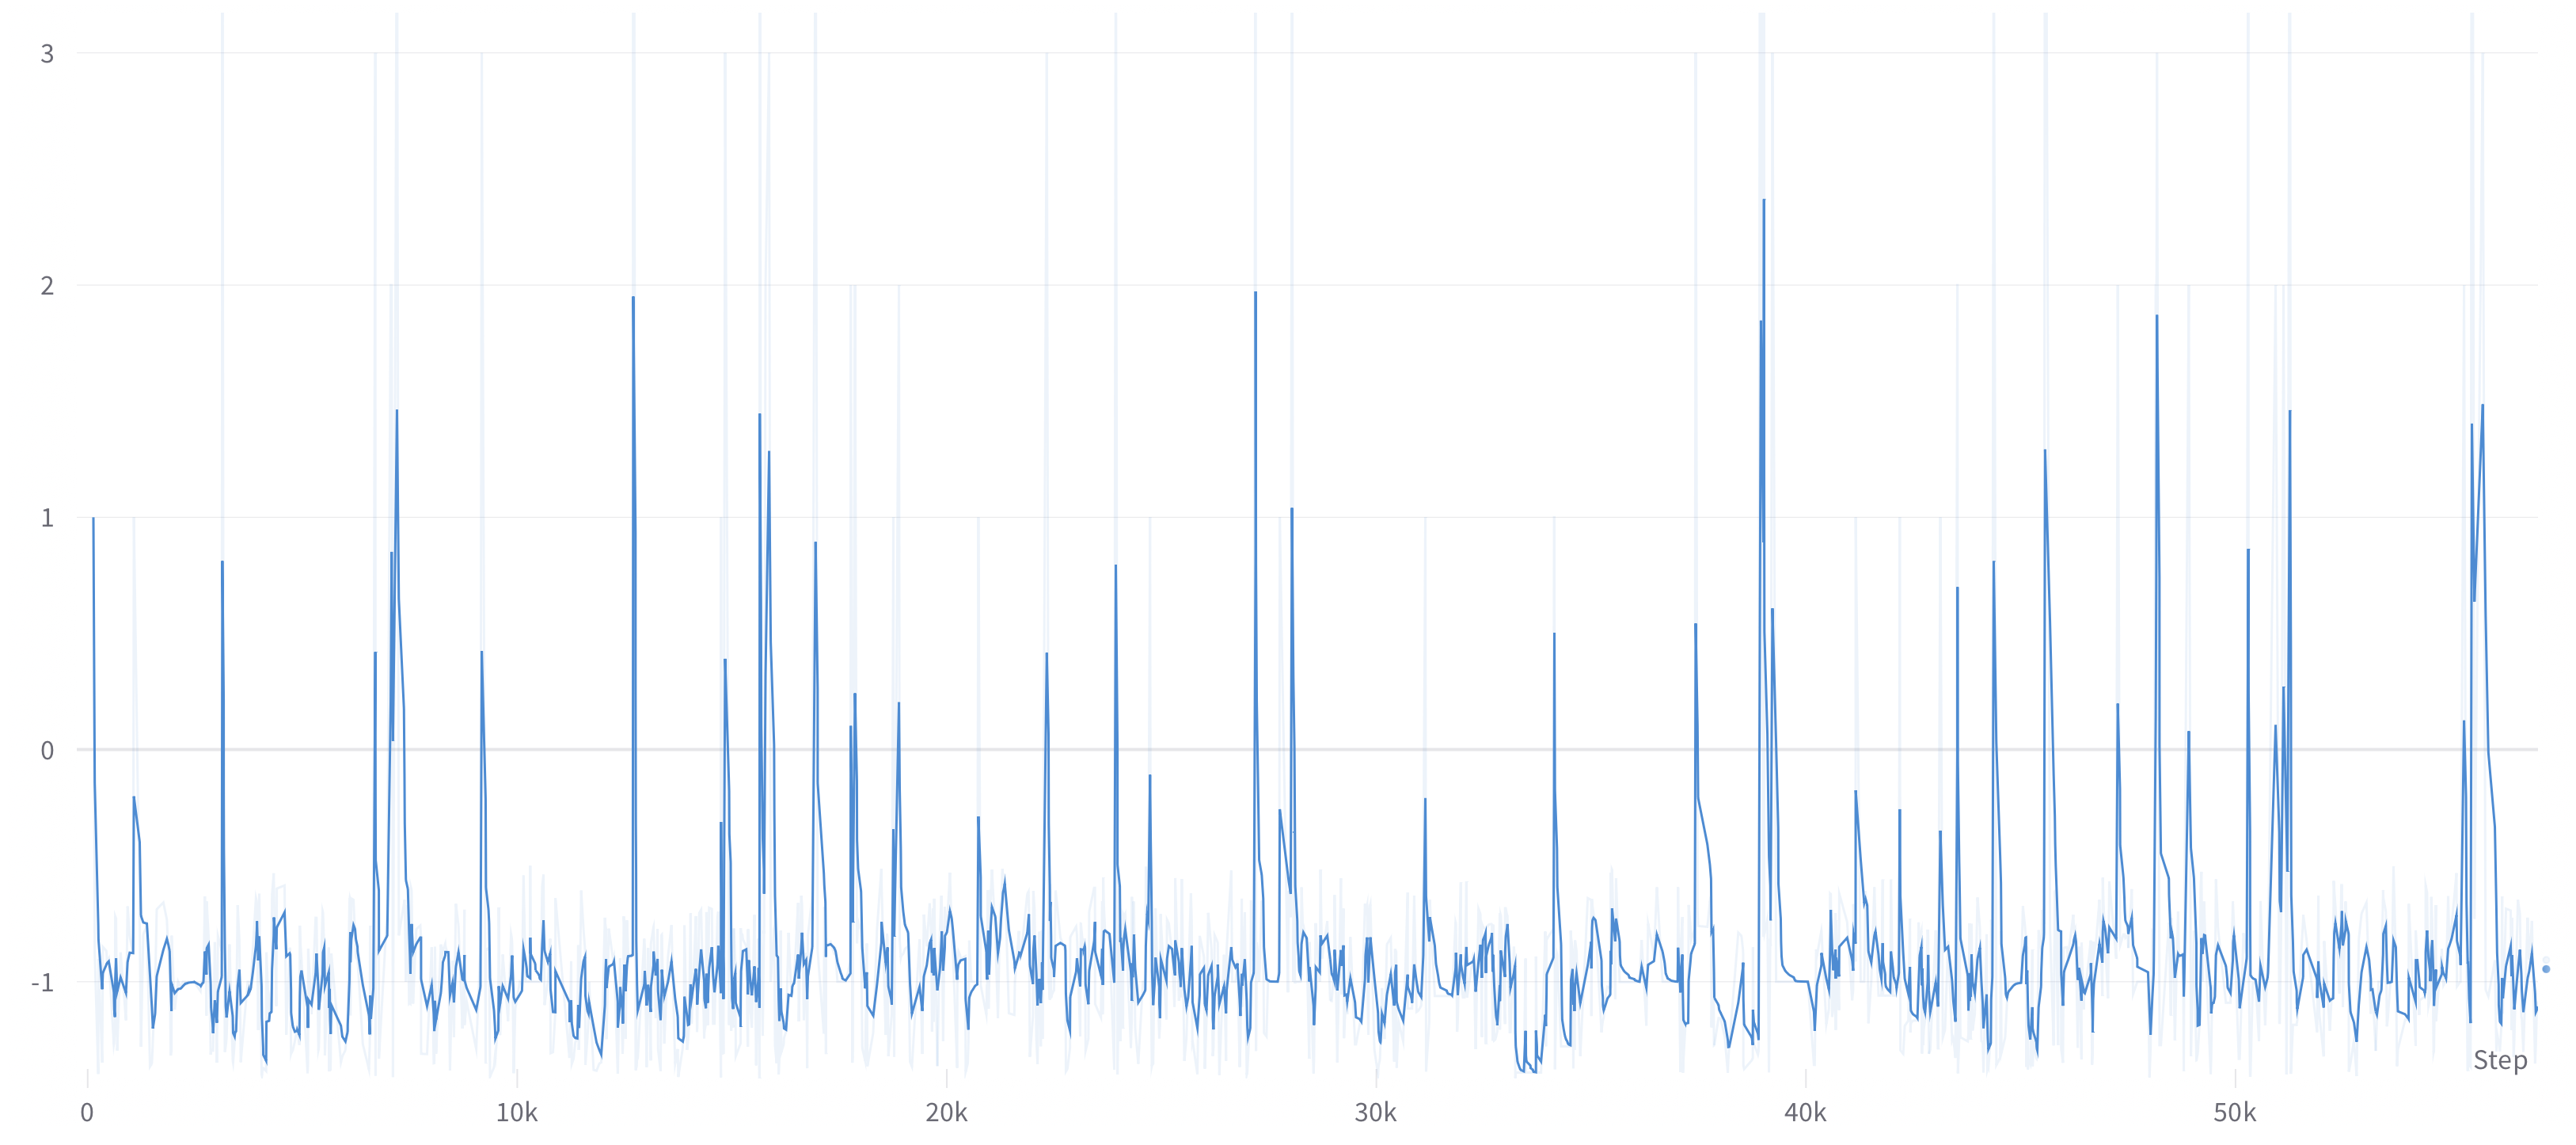
\includegraphics[width=\textwidth]{img/rewards_50_epochs.png}
      \caption{Total reward after 50 epochs}
      \label{fig:g}
  \end{subfigure}
  \hfill
  \begin{subfigure}[b]{0.45\textwidth}
      \centering
      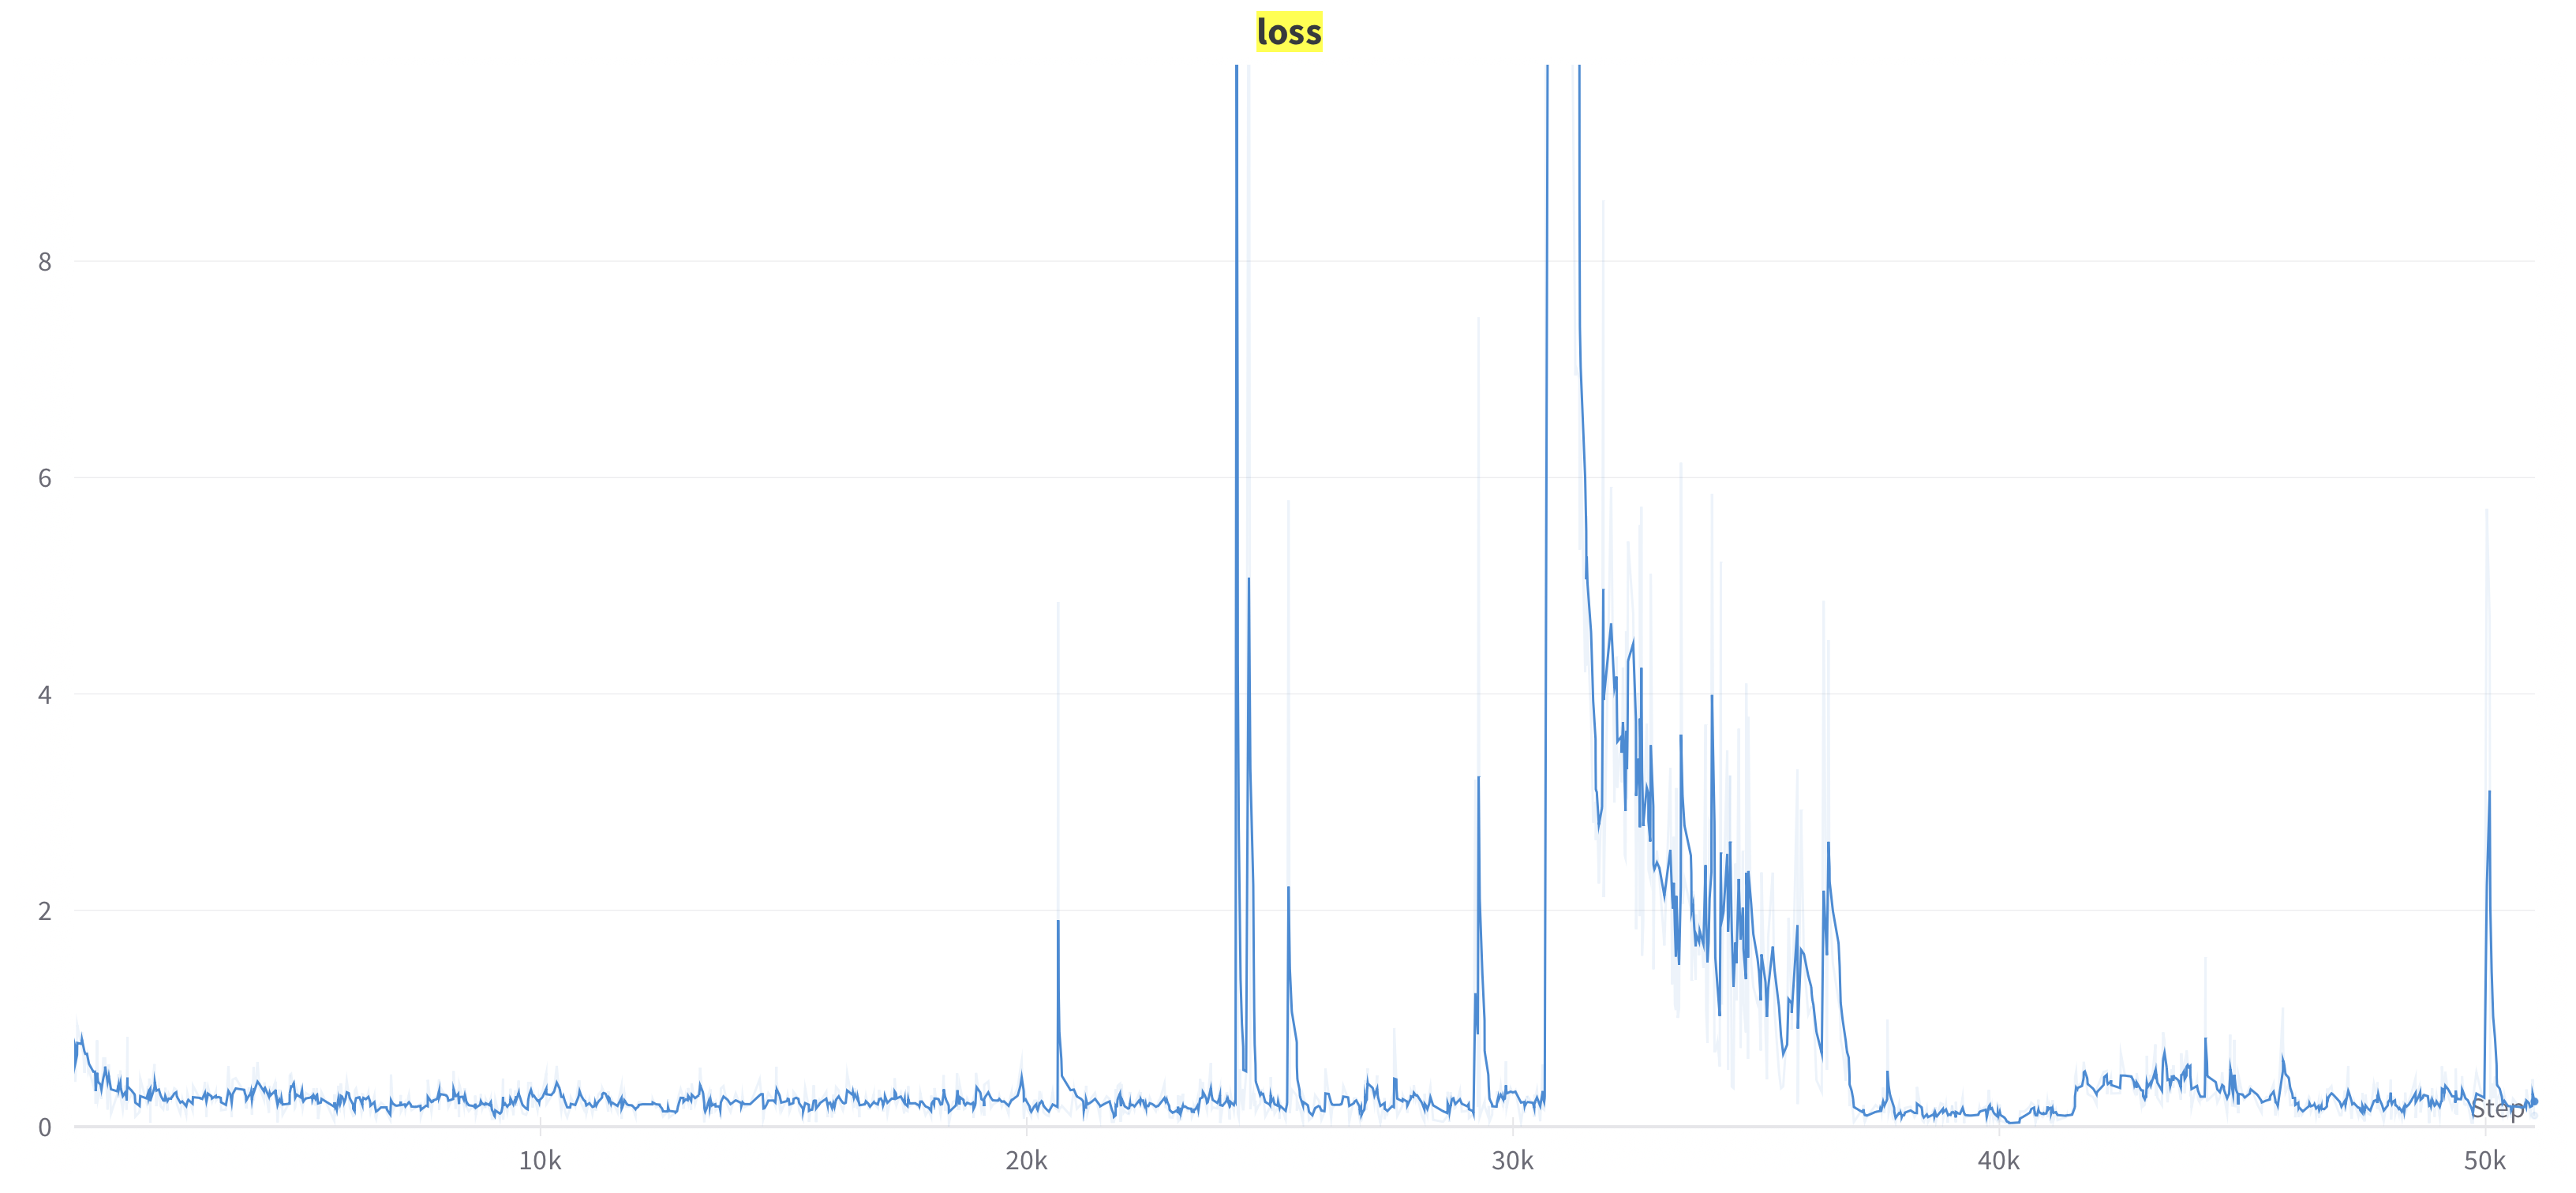
\includegraphics[width=\textwidth]{img/loss_50_epochs.png}
      \caption{Total loss after 50 epochs}
      \label{fig:h}
  \end{subfigure}
  \hfill
  \begin{subfigure}[b]{0.45\textwidth}
      \centering
      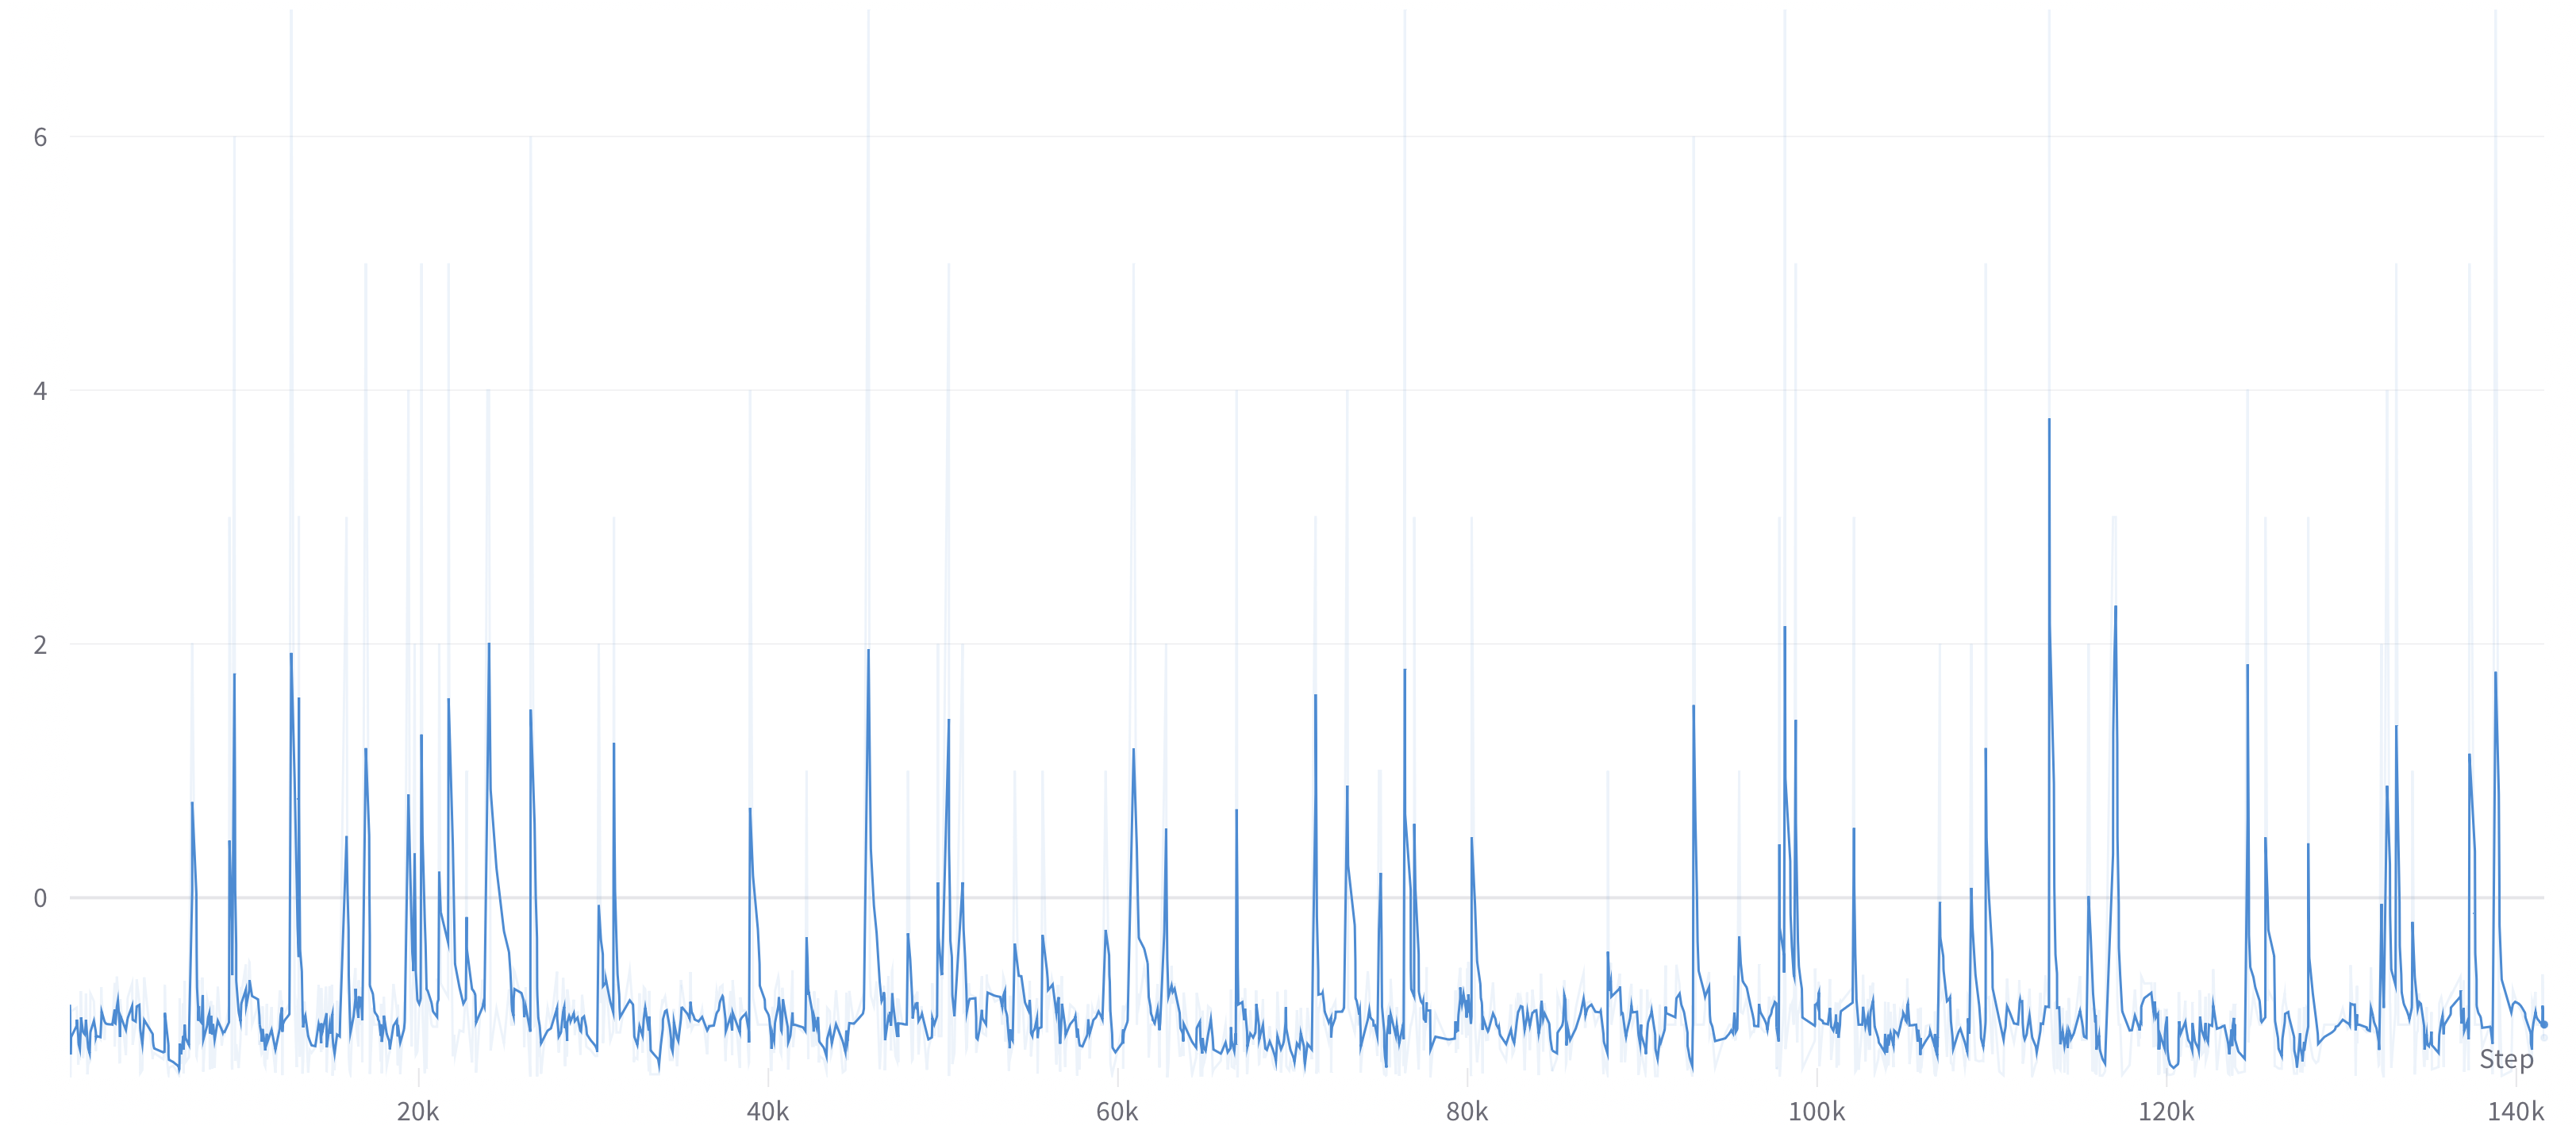
\includegraphics[width=\textwidth]{img/rewards.png}
      \caption{Total reward after 150 epochs} 
      \label{fig:i}
  \end{subfigure}
  \hfill
  \begin{subfigure}[b]{0.45\textwidth}
      \centering
      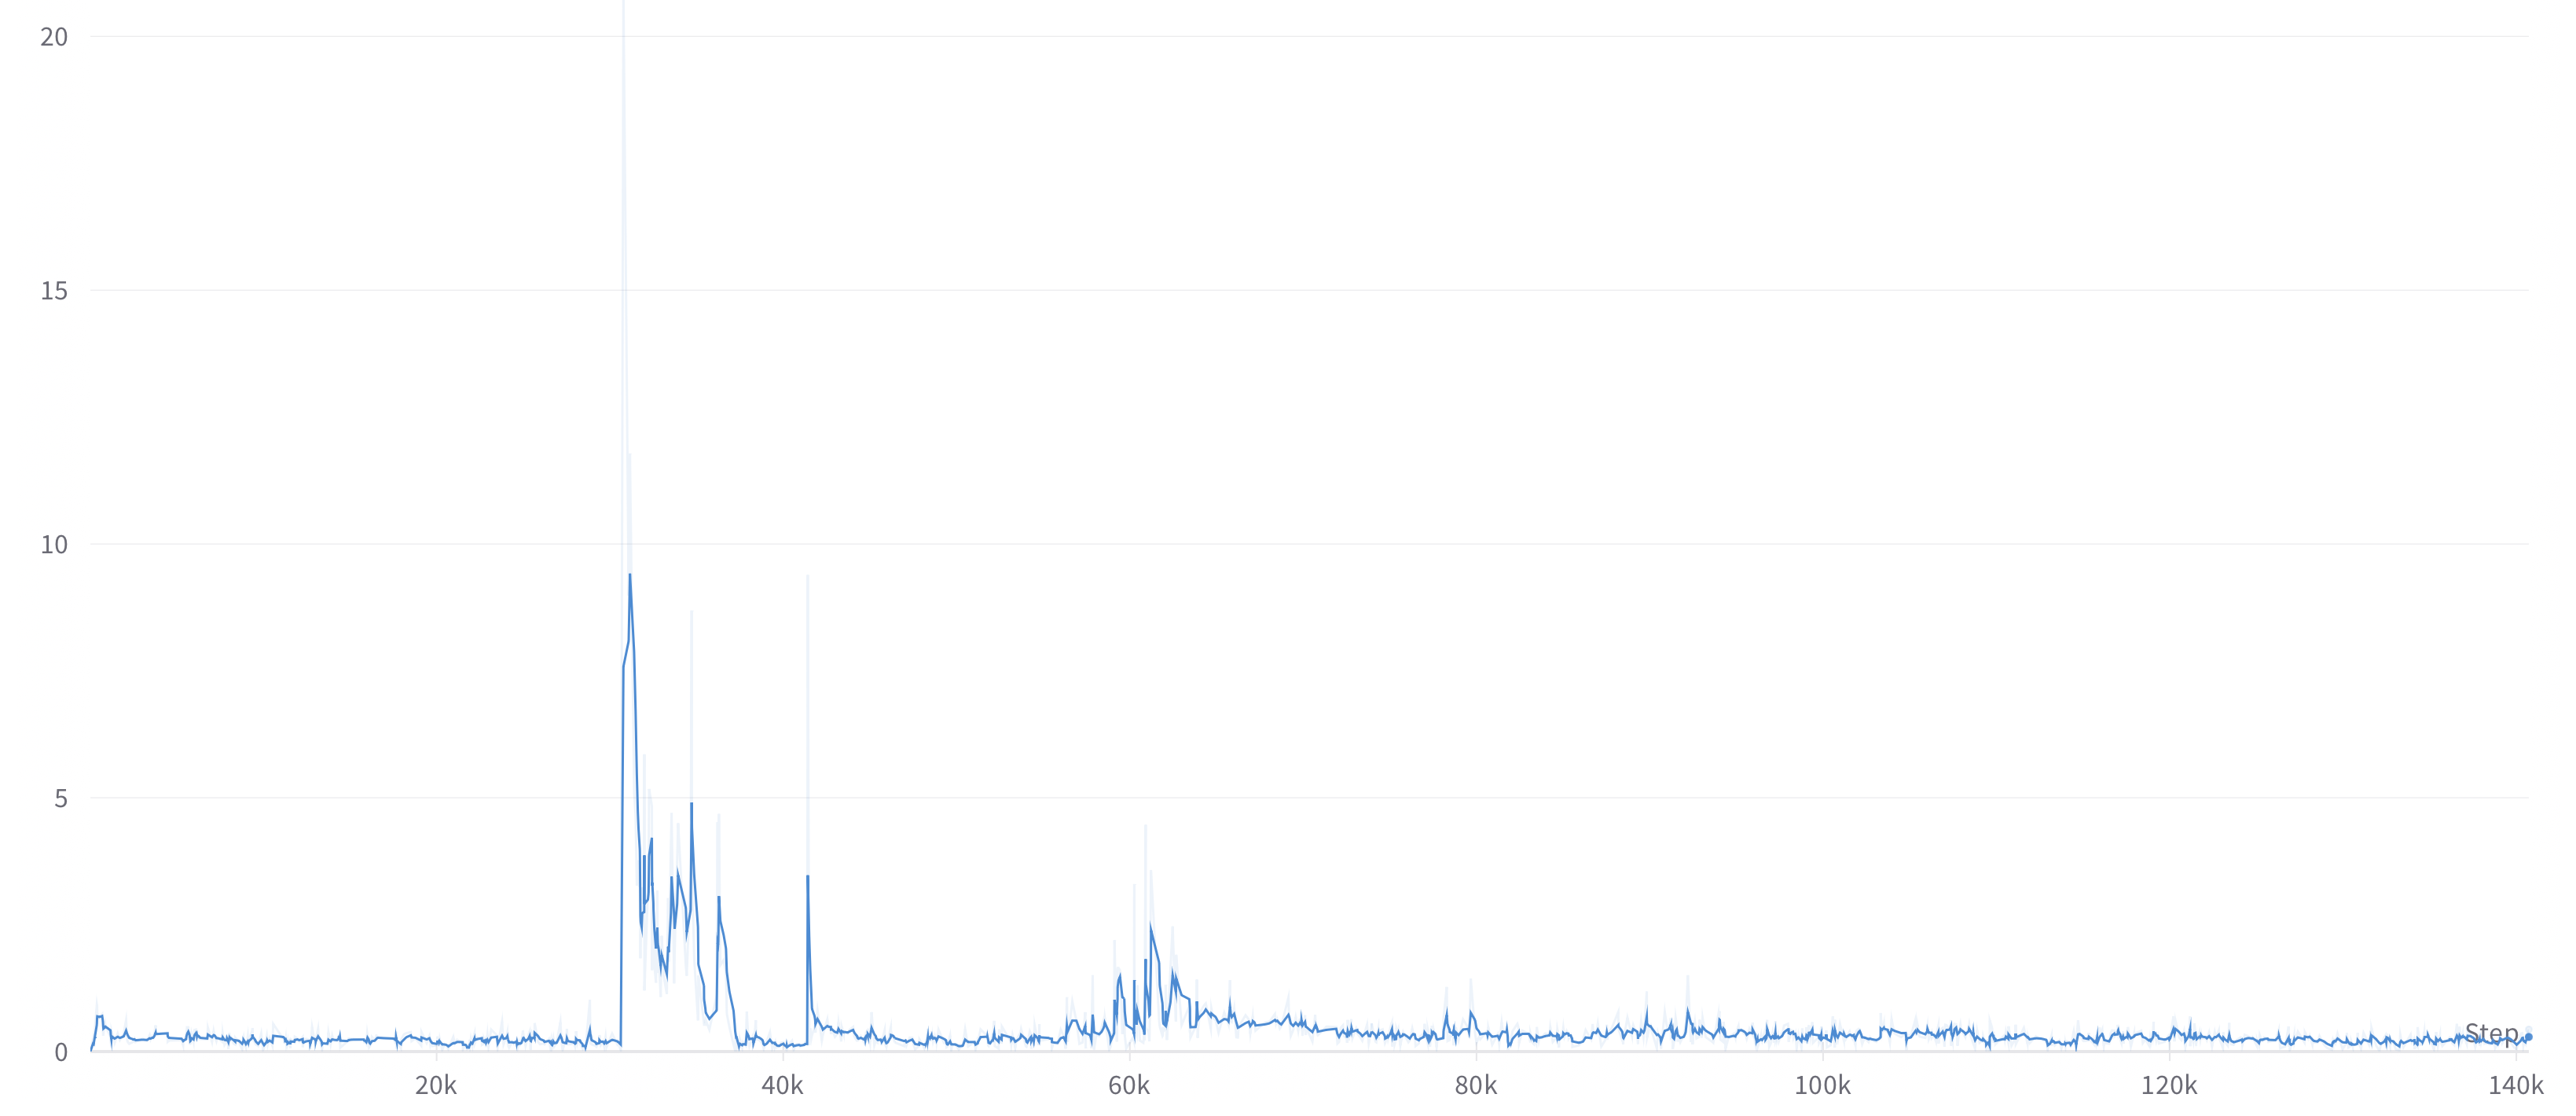
\includegraphics[width=\textwidth]{img/loss.png}
      \caption{Total loss after 150 epochs} 
      \label{fig:l}
  \end{subfigure}
  \caption{Reward and Loss comparison}
  \label{fig:s}
\end{figure}

During the initial epoch, agents exhibited limited familiarity with the task of removing targets from the 2D environment. Consequently, the mean reward achieved by the agents in this phase remained relatively low, with a maximum reward of approximately 3.0. As training progressed, agents displayed improved performance [\ref{fig:g}]. By the 70th epoch, the highest recorded mean reward reached 8.0, typically occurring at around 900 steps into the episode. This milestone indicated that agents had grasped the fundamentals of their task but still had room for refinement.

A significant leap in performance was observed at the 145th epoch [\ref{fig:i}]. Agents demonstrated remarkable efficiency by removing almost all targets in fewer than 500 steps, with the last remaining target eliminated in the final steps of the episode. Concurrently, the loss function exhibited a notable pattern. While initially showing spikes when agents were rewarded values exceeding 1.0 [\ref{fig:h}], the loss gradually minimized and stabilized near zero after the 100th epoch [\ref{fig:l}].

\begin{figure}
  \centering
  \begin{subfigure}[b]{0.45\textwidth}
      \centering
      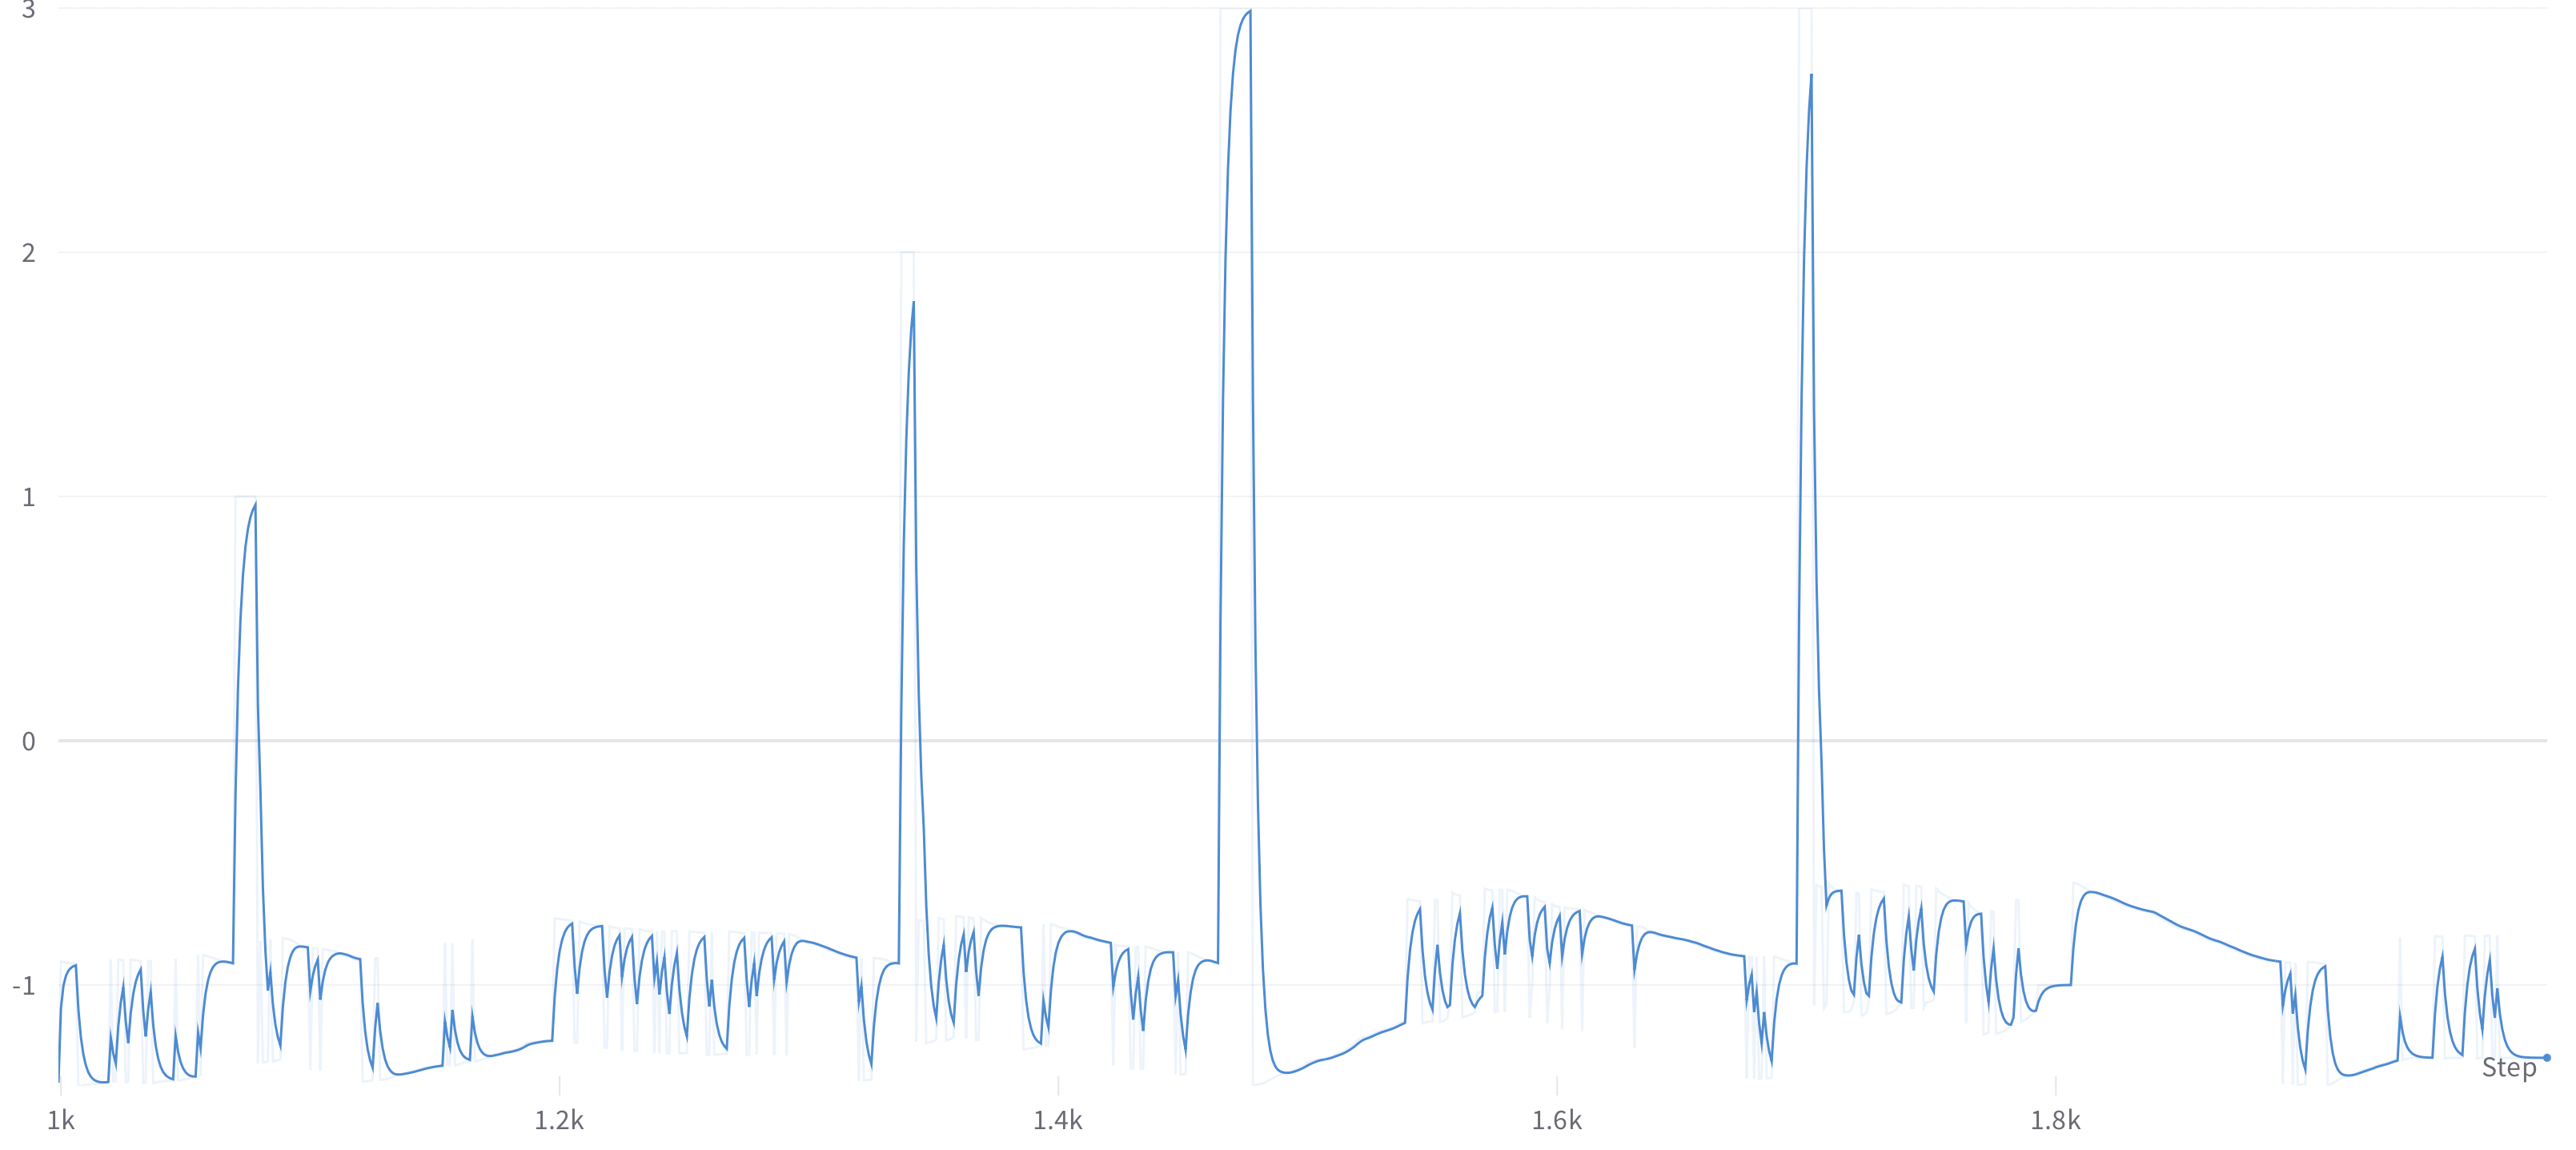
\includegraphics[width=\textwidth]{img/mean_reward_1_epoch.png}
      \caption{Mean Reward Epoch 1}
      \label{fig:d}
  \end{subfigure}
  \hfill
  \begin{subfigure}[b]{0.45\textwidth}
      \centering
      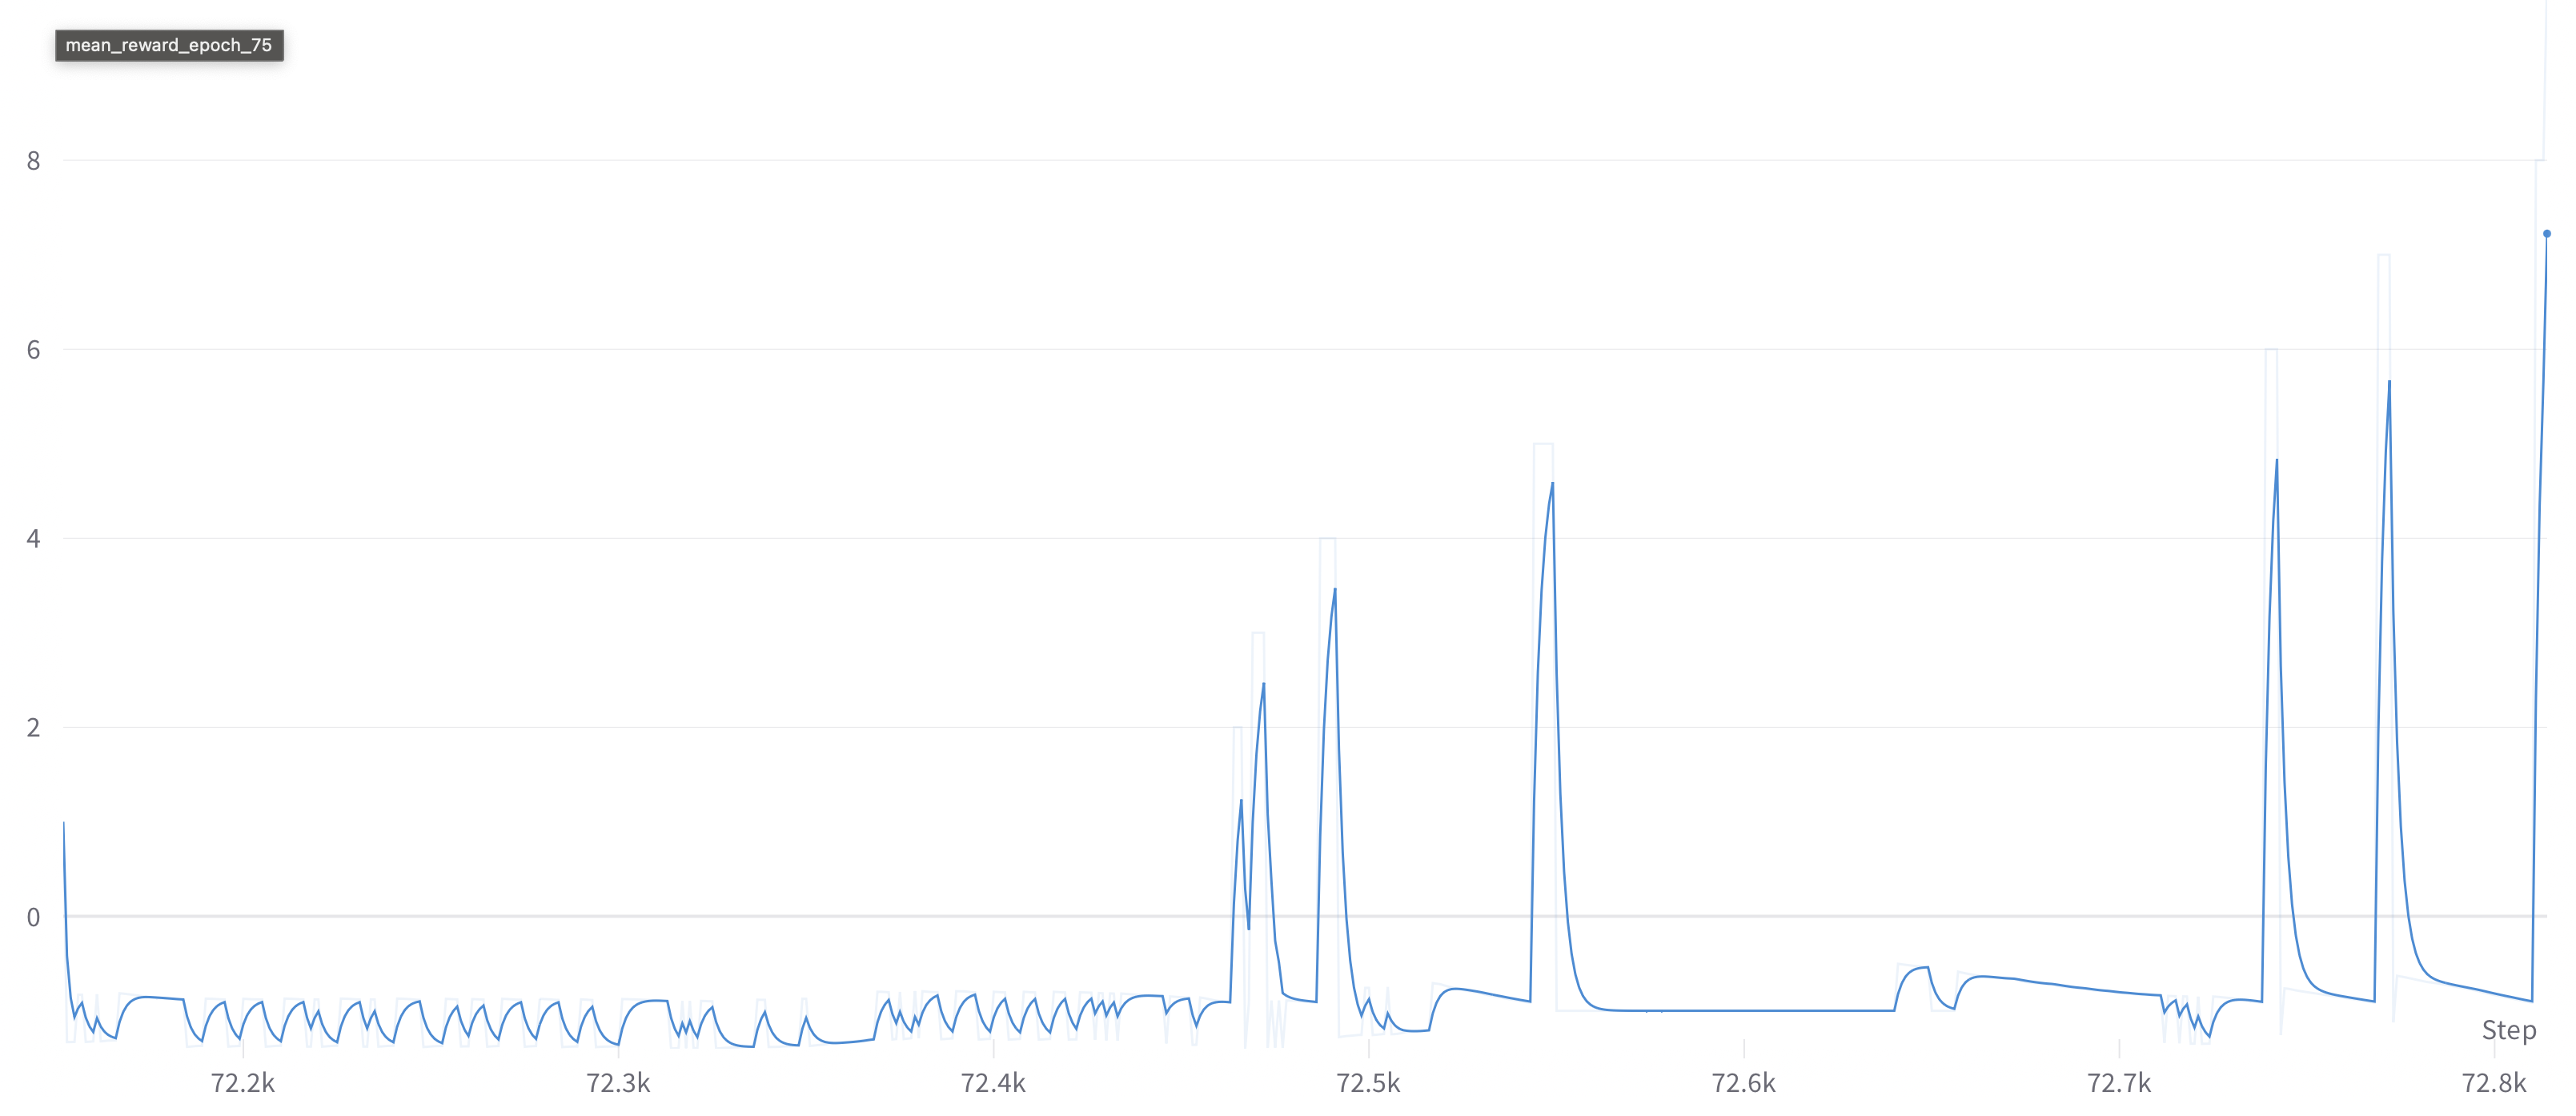
\includegraphics[width=\textwidth]{img/mean_reward_70_epoch.png}
      \caption{Mean Reward Epoch 70}
      \label{fig:e}
  \end{subfigure}
  \hfill
  \begin{subfigure}[b]{0.45\textwidth}
      \centering
      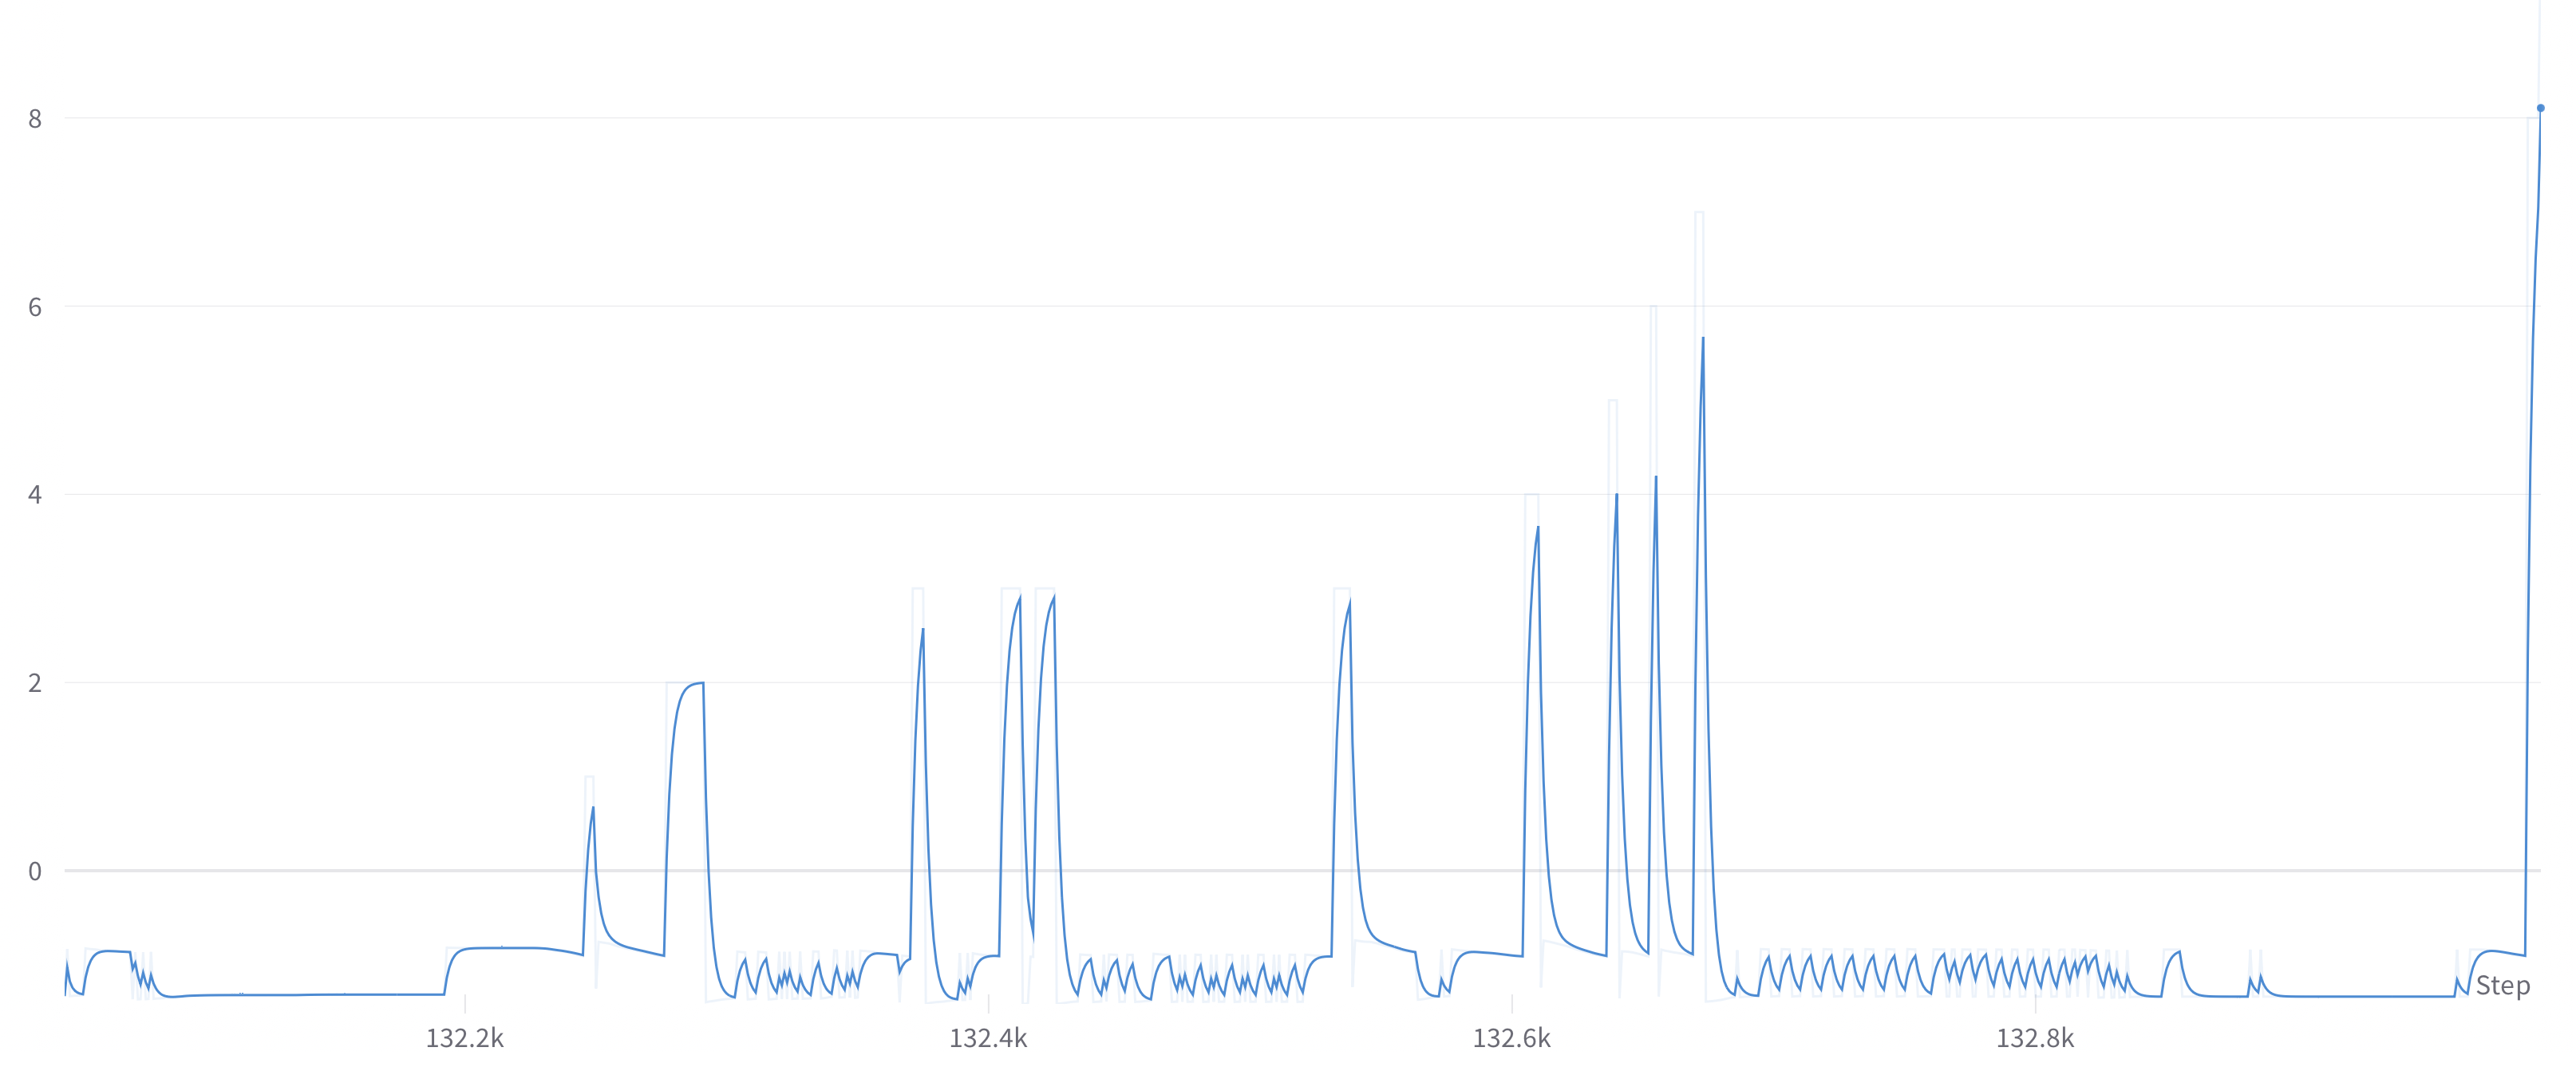
\includegraphics[width=\textwidth]{img/mean_reward_145_epoch.png}
      \caption{Mean Reward Epoch 145} 
      \label{fig:f}
  \end{subfigure}
  \caption{Mean rewards}
\end{figure}

\subsubsection{Evaluation Results}

\begin{figure}
  \centering
  \begin{subfigure}[b]{0.45\textwidth}
      \centering
      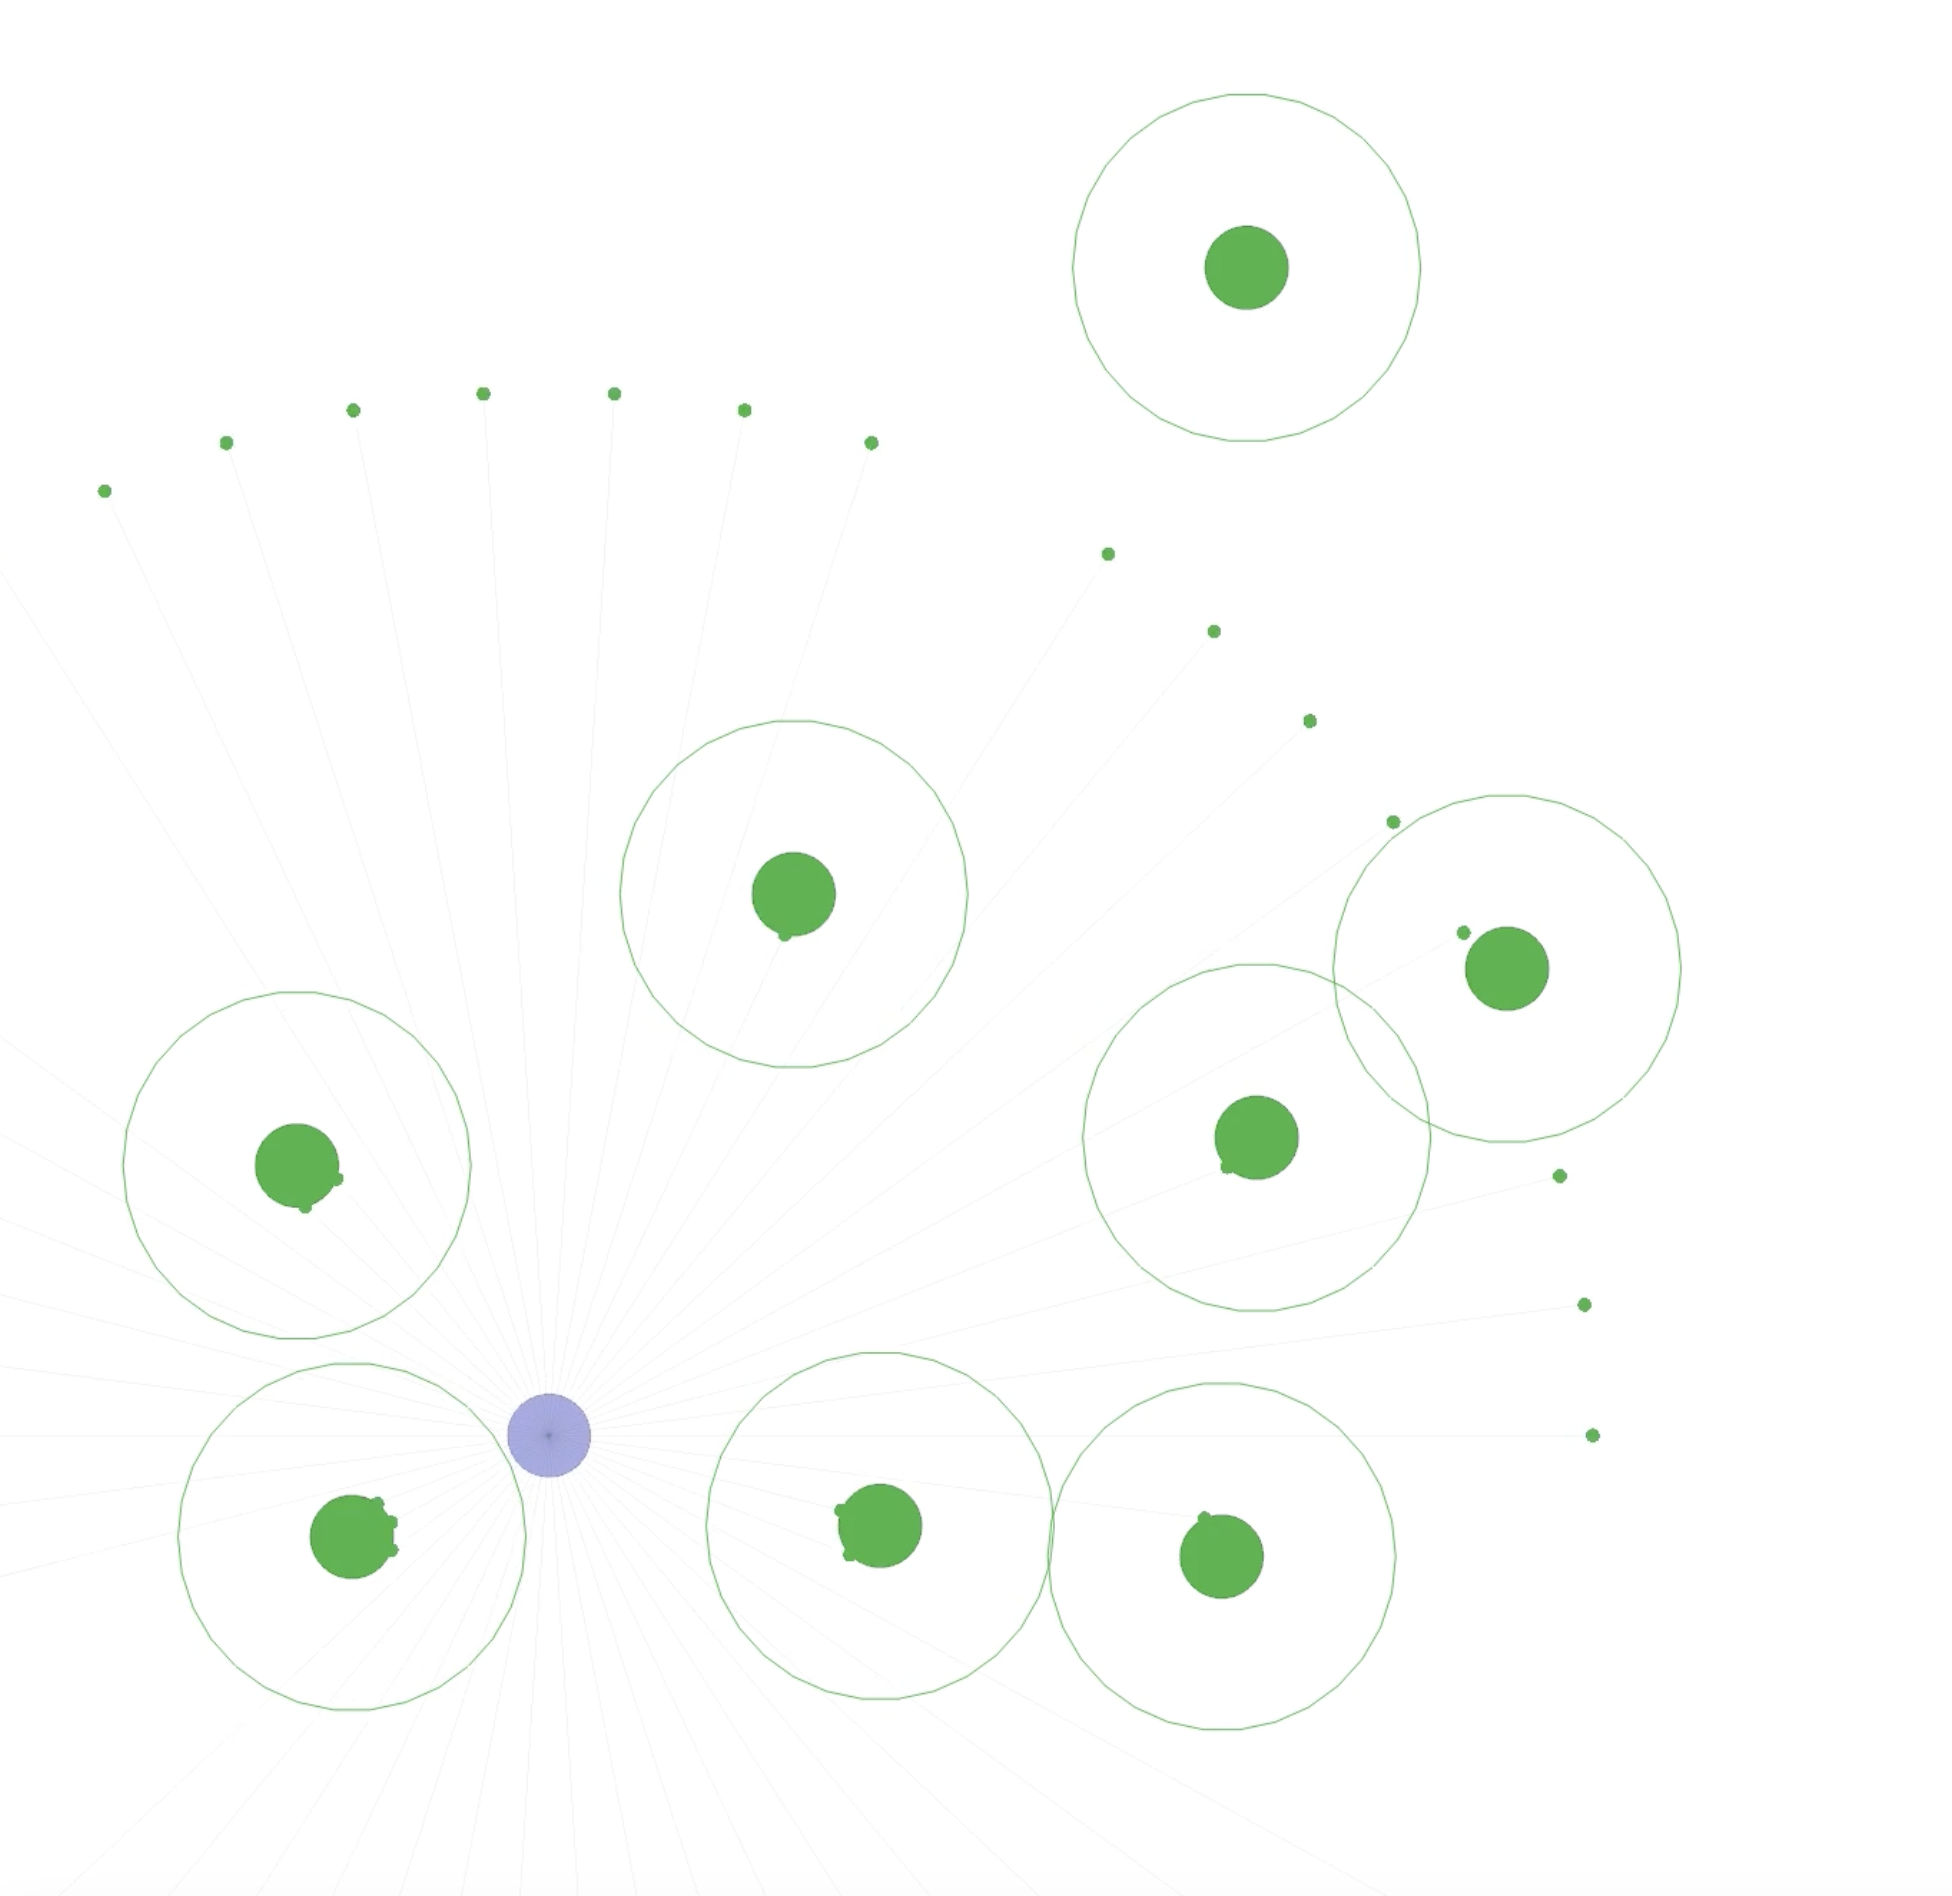
\includegraphics[width=\textwidth]{img/1_agent_1.png}
      \caption{Beginning of simulation}
  \end{subfigure}
  \hfill
  \begin{subfigure}[b]{0.45\textwidth}
      \centering
      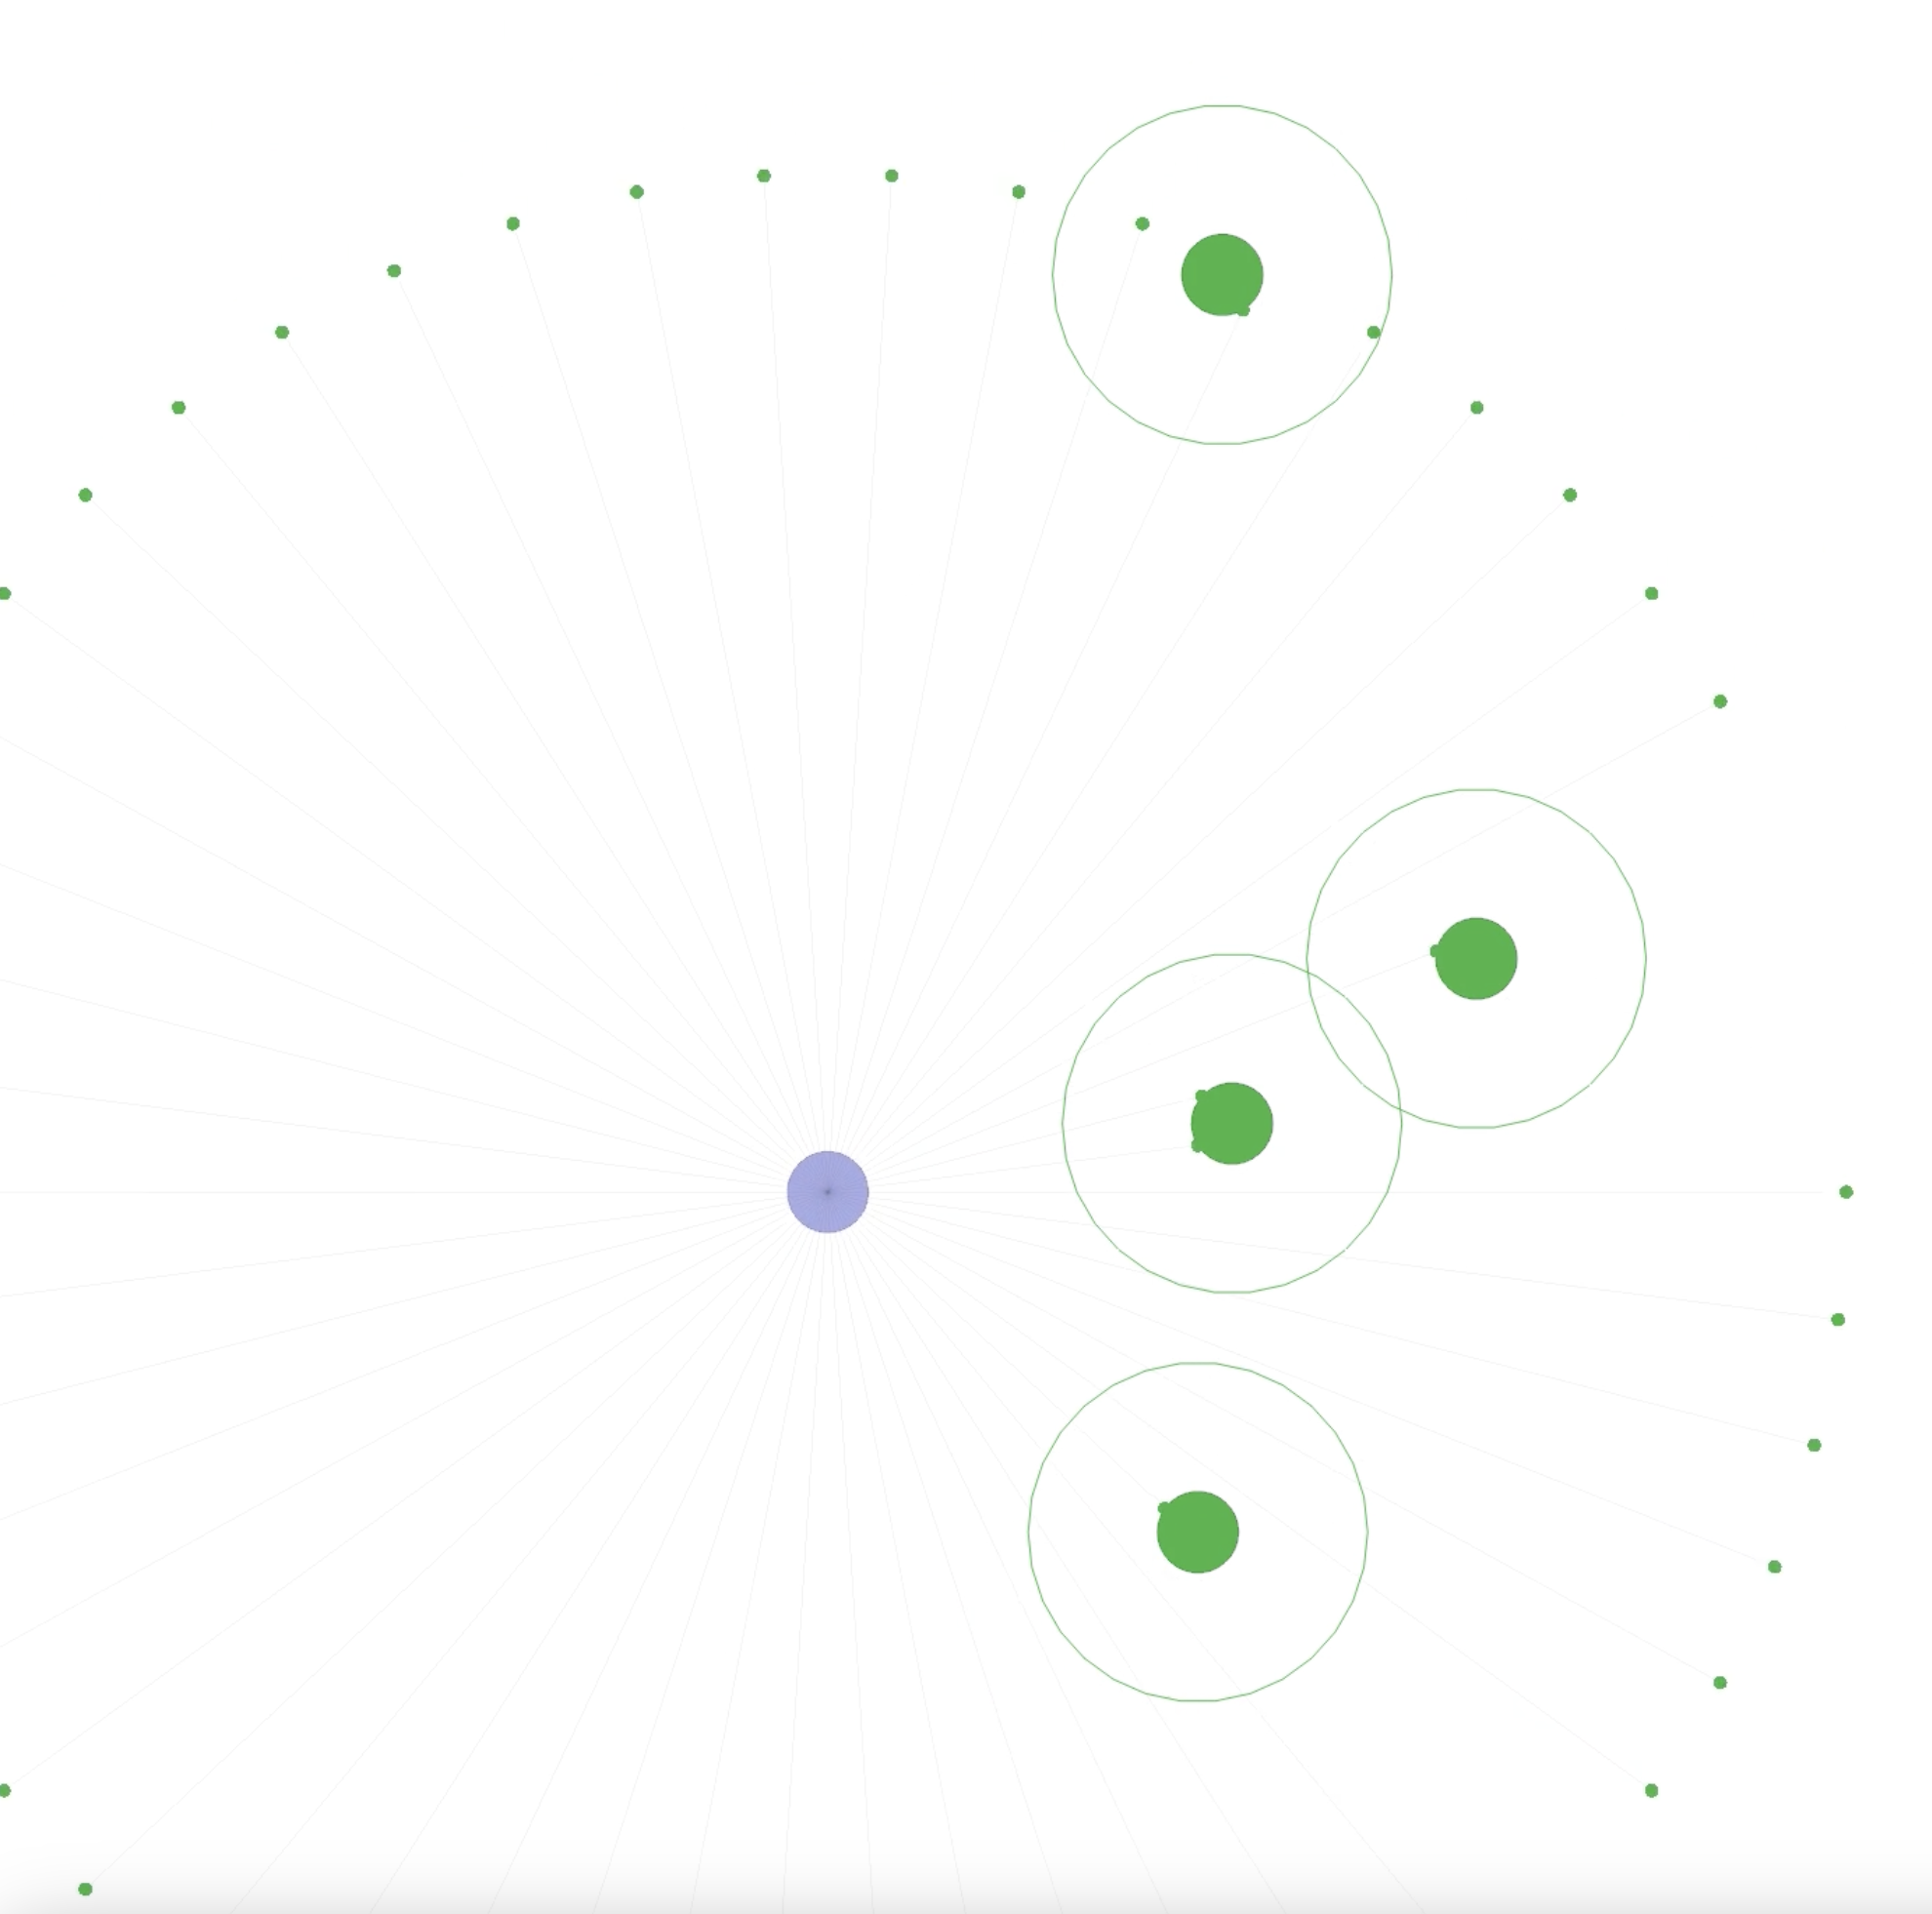
\includegraphics[width=\textwidth]{img/1_agent_2.png}
      \caption{Half simulation}
  \end{subfigure}
  \hfill
  \begin{subfigure}[b]{0.45\textwidth}
      \centering
      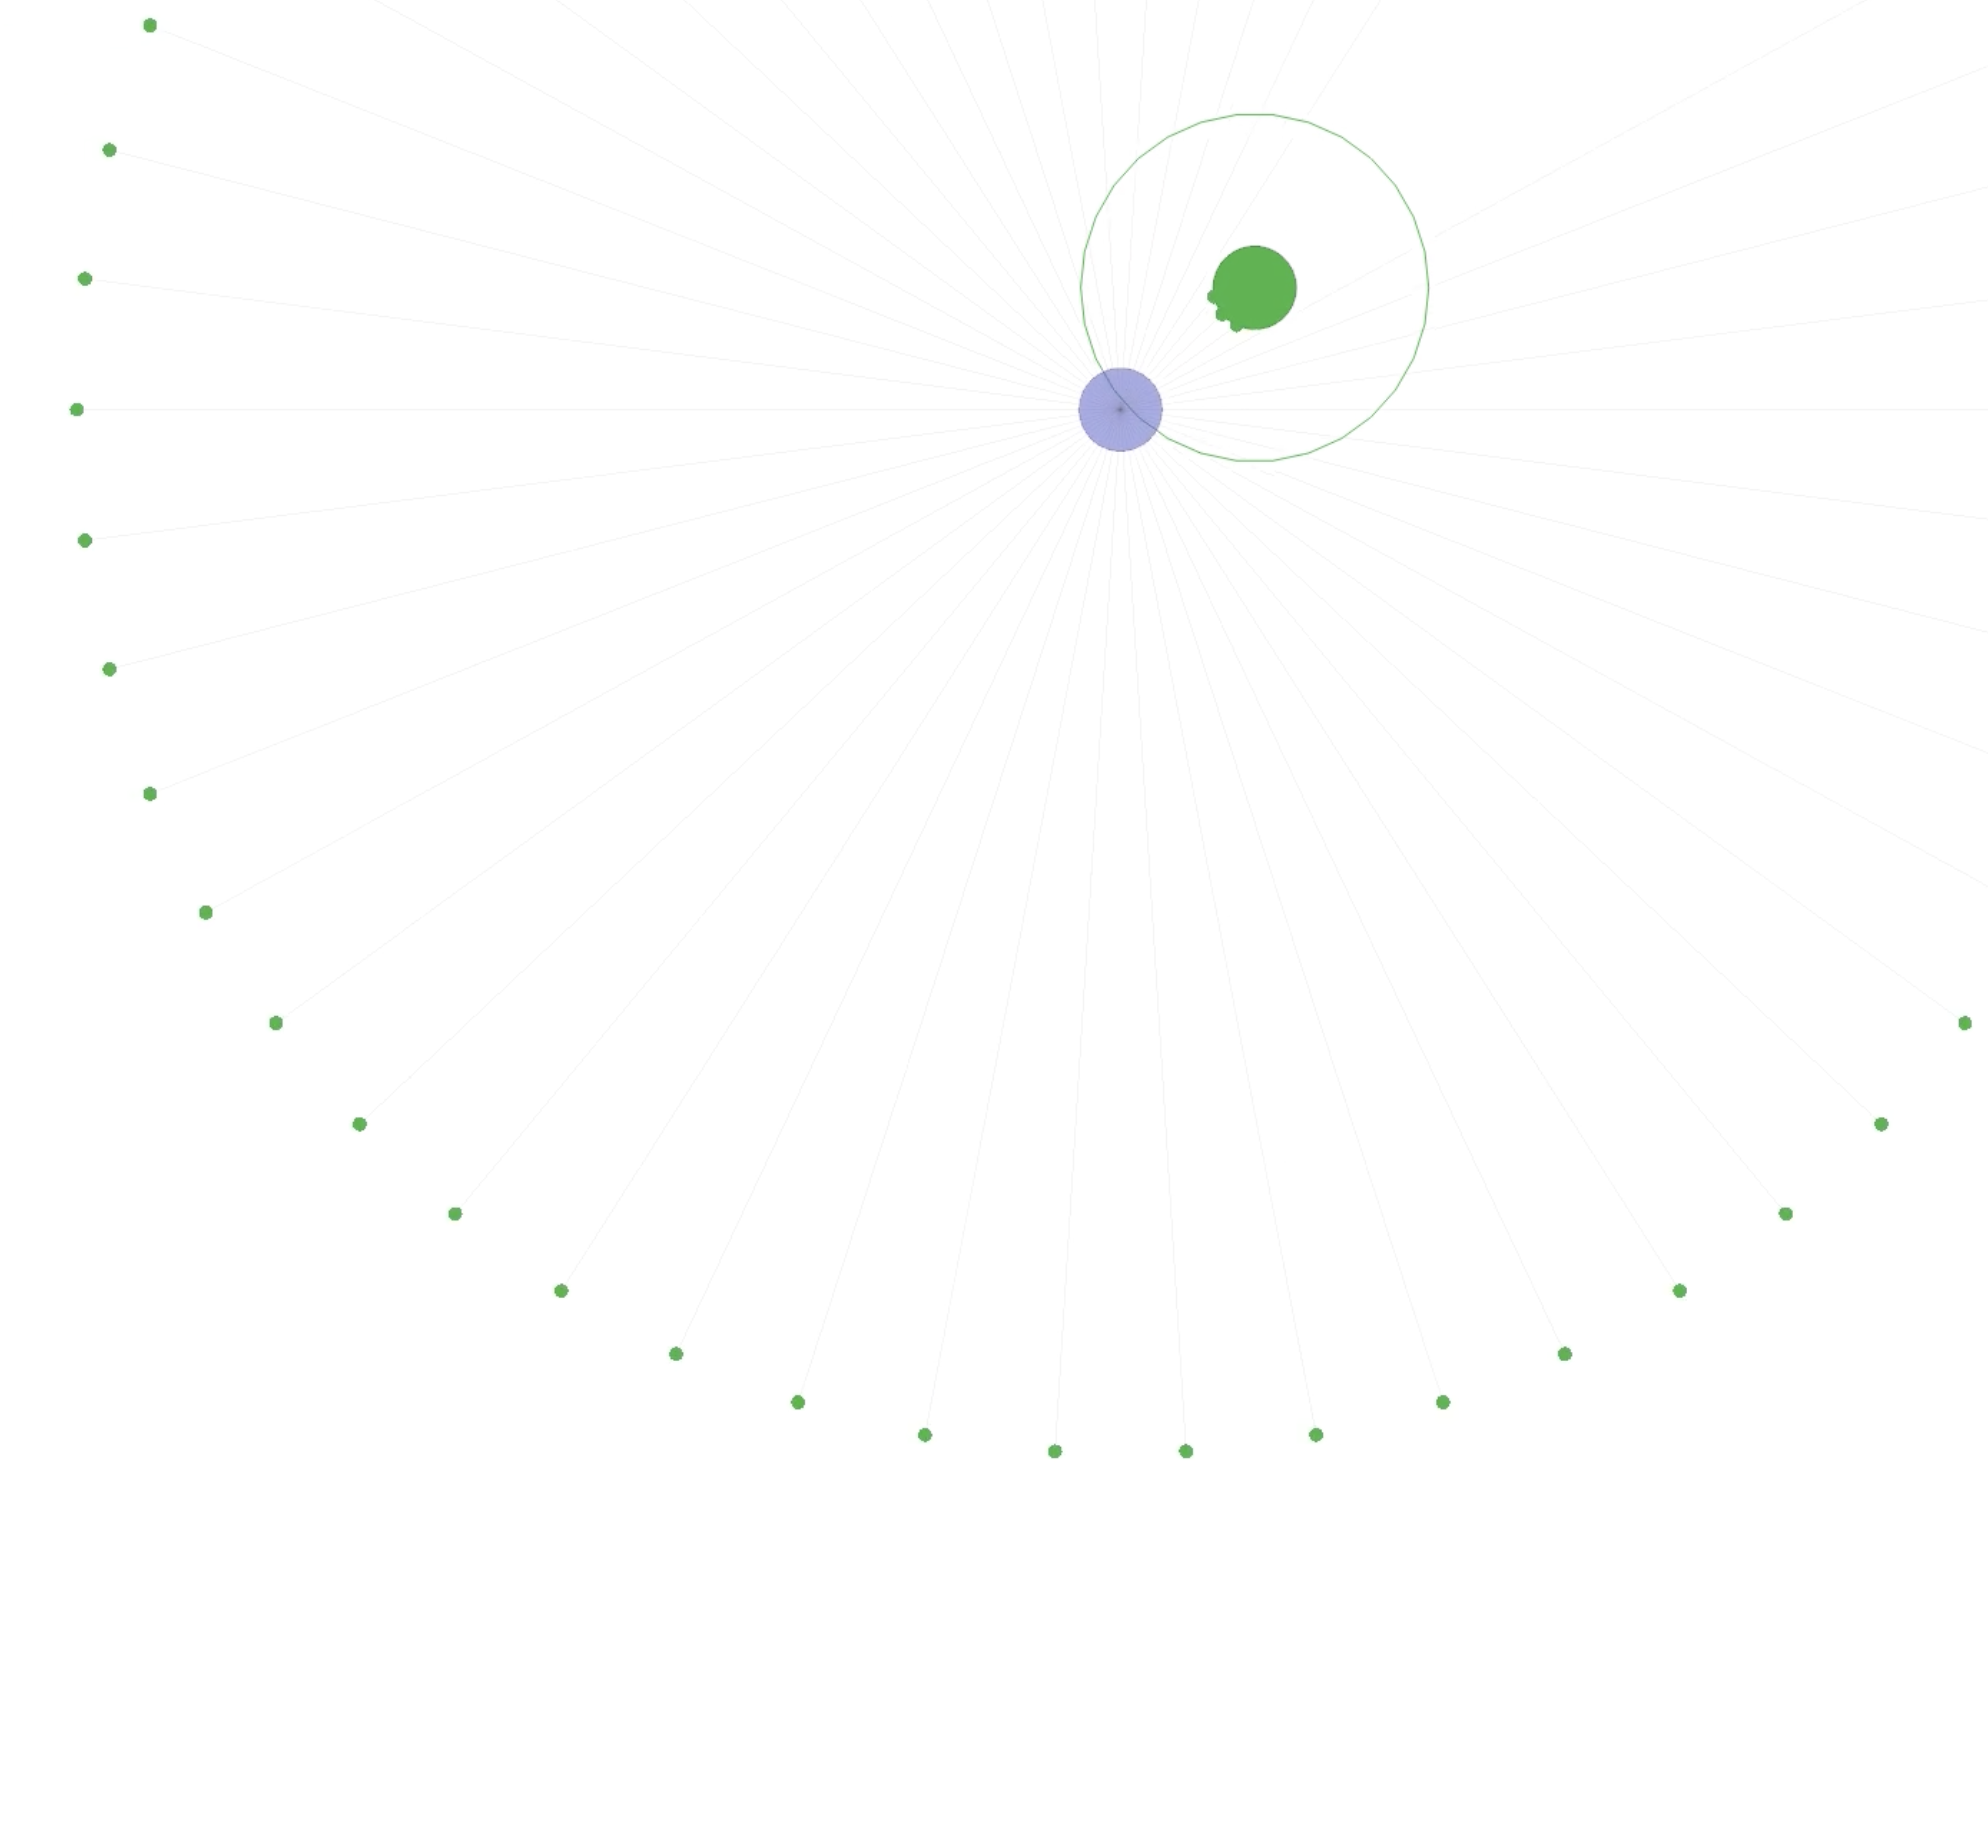
\includegraphics[width=\textwidth]{img/1_agent_3.png}
      \caption{End of simulation} 
  \end{subfigure}
  \caption{Different stages of a simulation with one agent and 8 targets}
  \label{fig:m}
\end{figure}

To assess the agents' performance in practical scenarios, I conducted evaluations with varying numbers of agents and targets. In a scenario involving one agent and eight targets [\ref{fig:m}], the results indicated the following:
\begin{itemize}
  \item On average, it took approximately 10 steps for the agent to remove the first target, reflecting a quick initiation of the cleaning process [\ref{fig:d}].
  \item Removal of half the targets occurred, on average, in approximately 170 steps, demonstrating consistent progress [\ref{fig:e}].
  \item To remove all eight targets, agents required an average of around 1440 steps, highlighting the complexity of clearing the entire environment [\ref{fig:f}].
\end{itemize}

\begin{figure}
  \centering
  \begin{subfigure}[b]{0.45\textwidth}
      \centering
      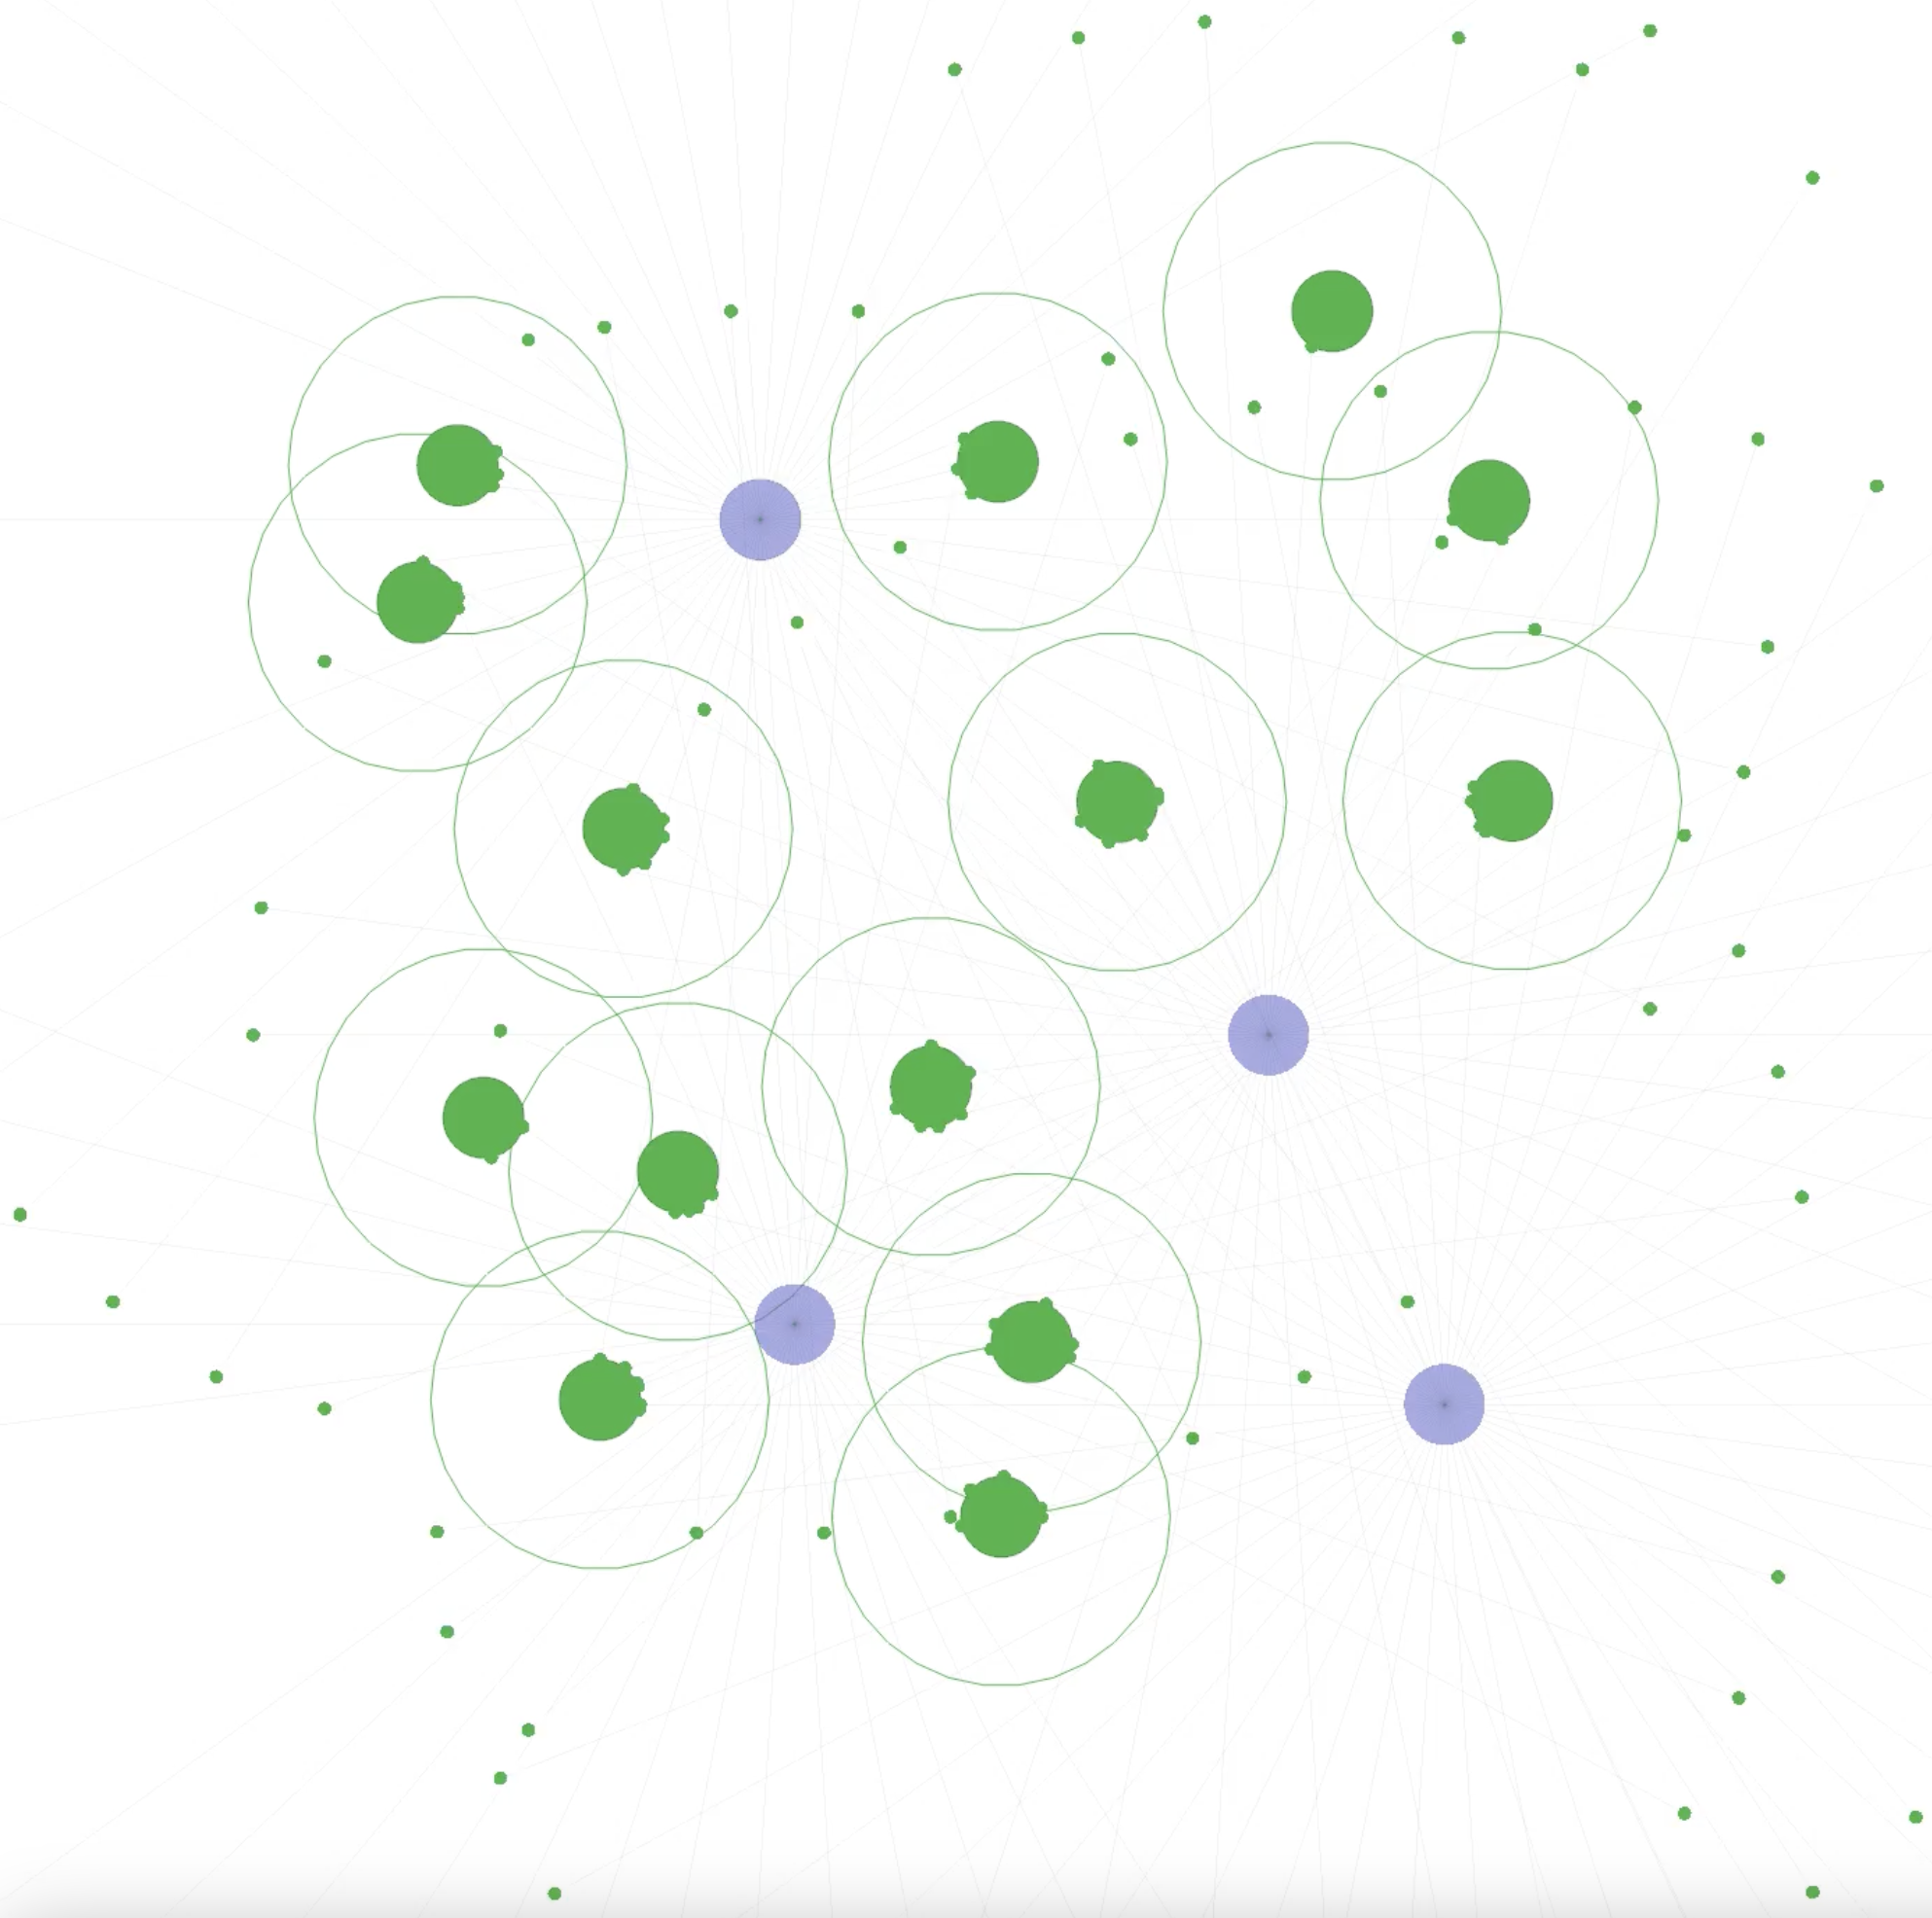
\includegraphics[width=\textwidth]{img/4_agents_1.png}
      \caption{Beginning of simulation}
  \end{subfigure}
  \hfill
  \begin{subfigure}[b]{0.45\textwidth}
      \centering
      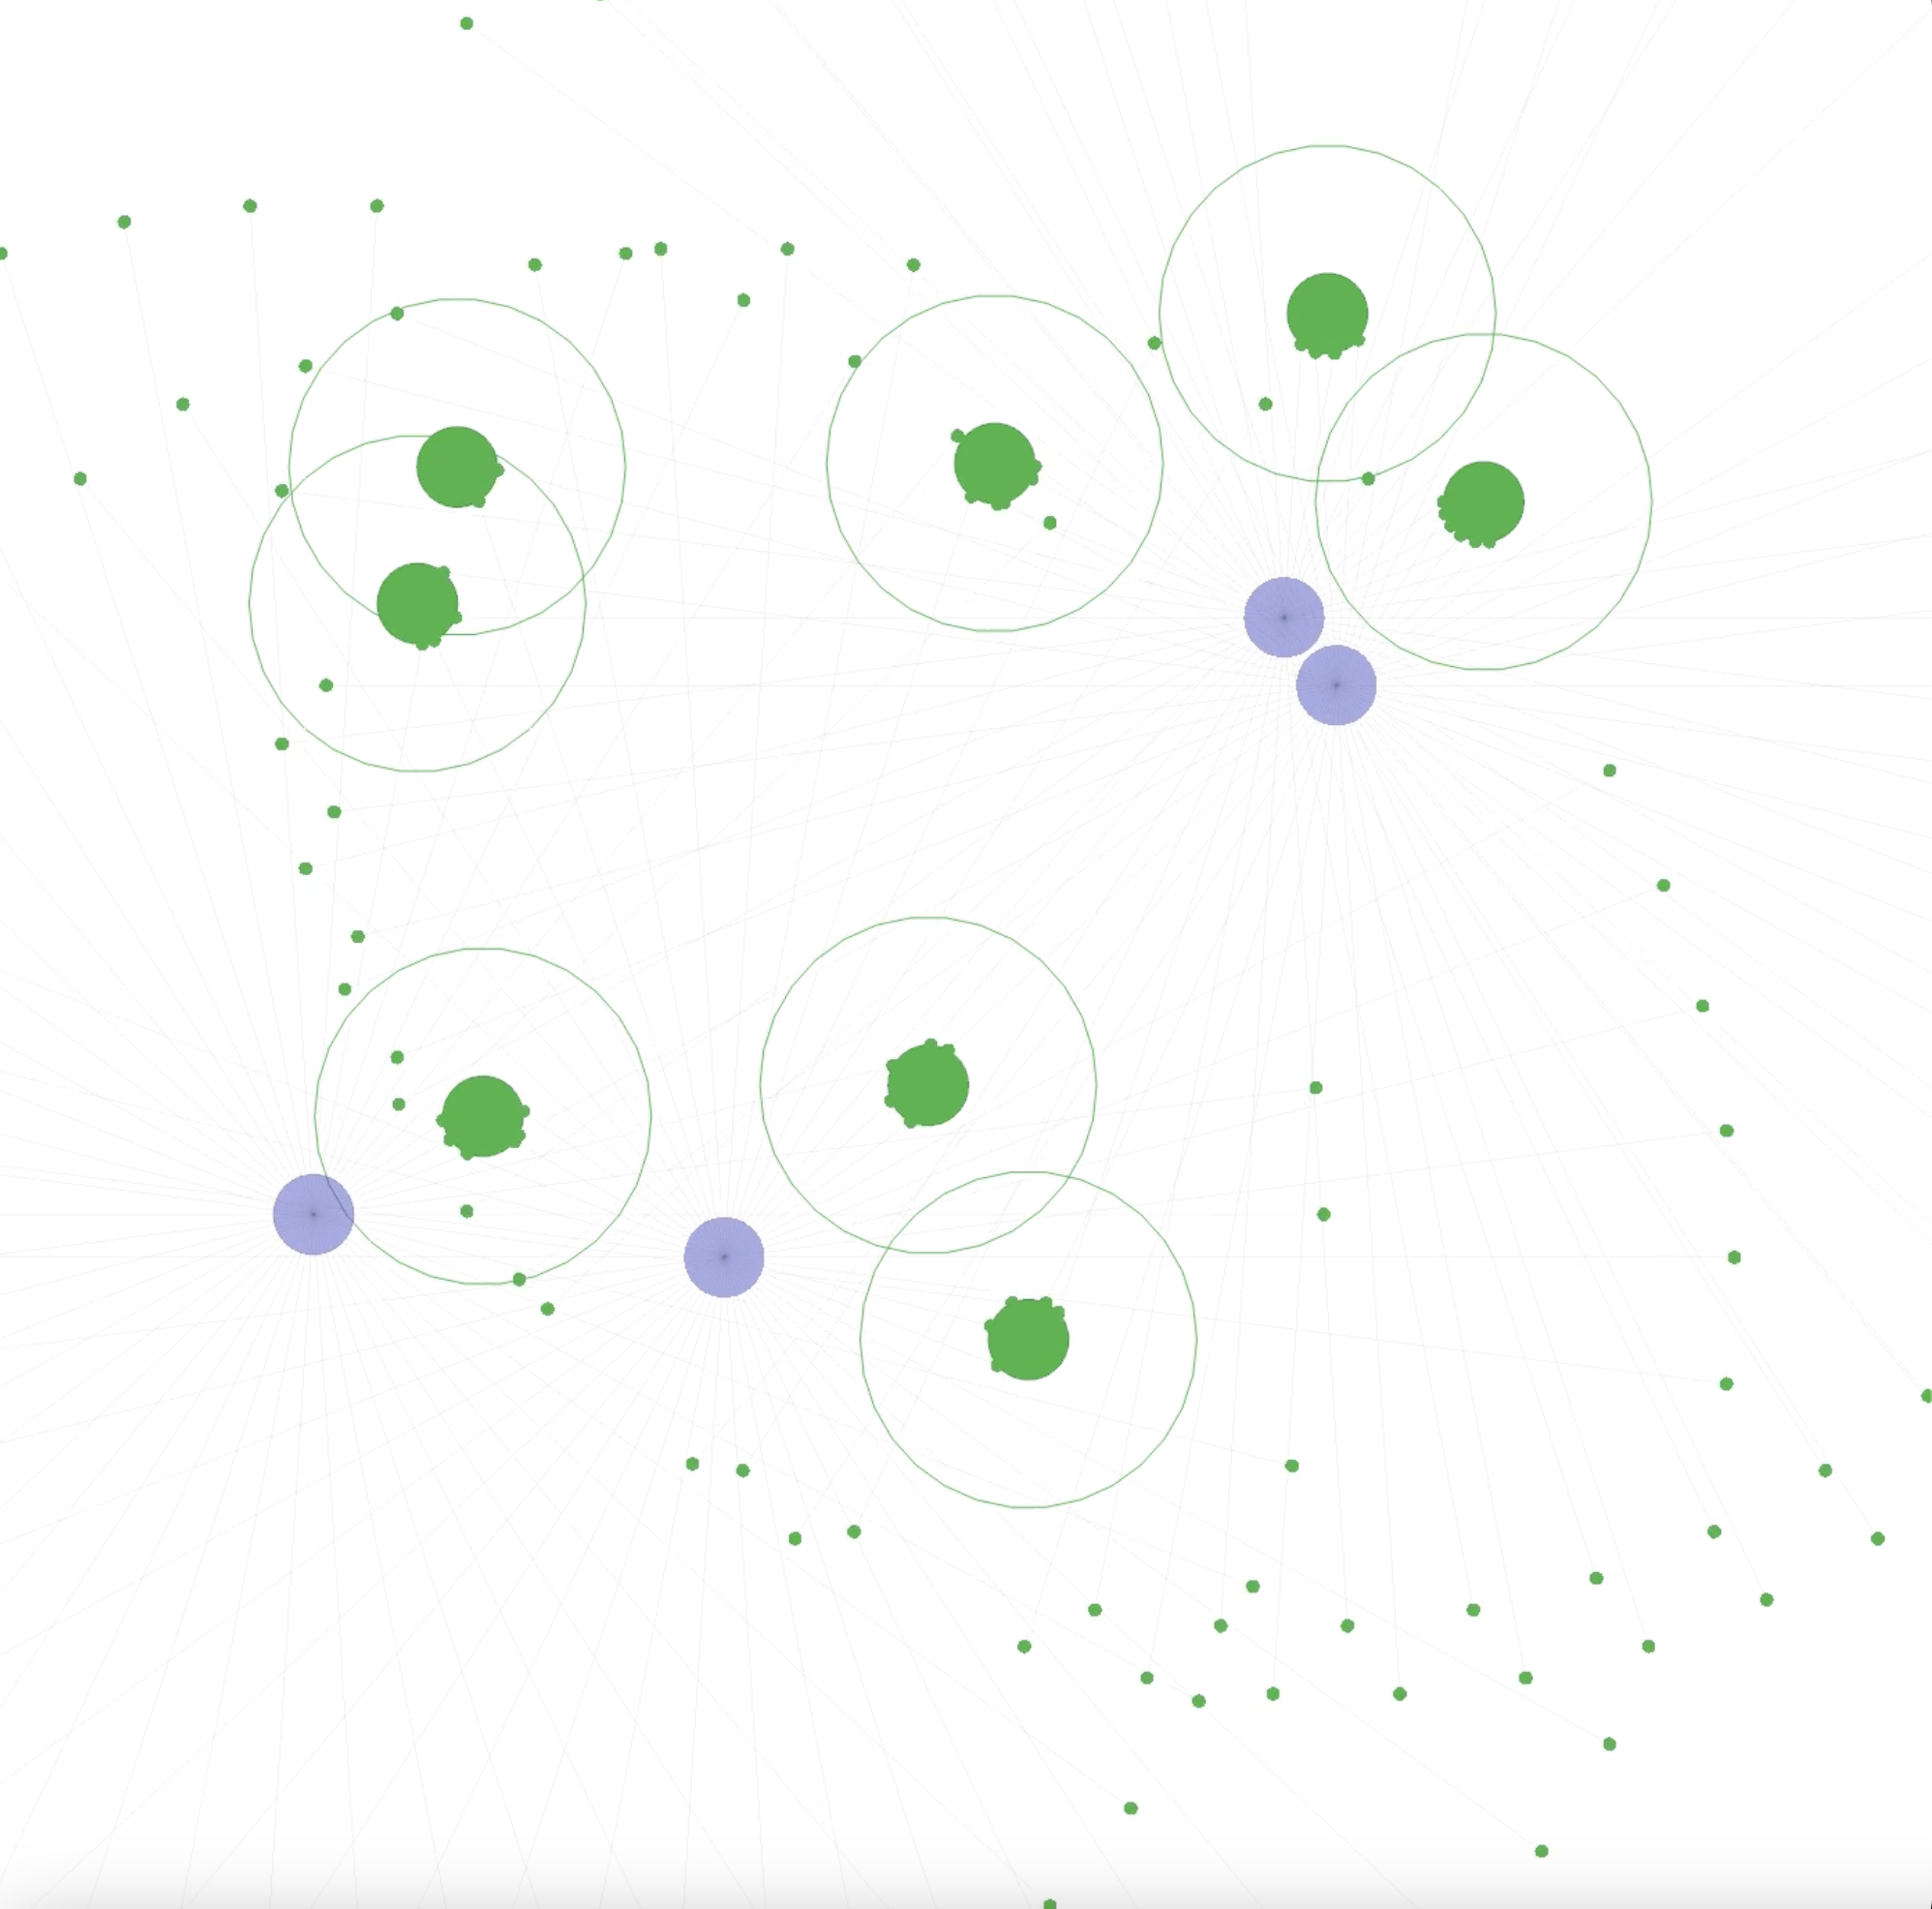
\includegraphics[width=\textwidth]{img/4_agents_2.png}
      \caption{Half simulation}
  \end{subfigure}
  \hfill
  \begin{subfigure}[b]{0.45\textwidth}
      \centering
      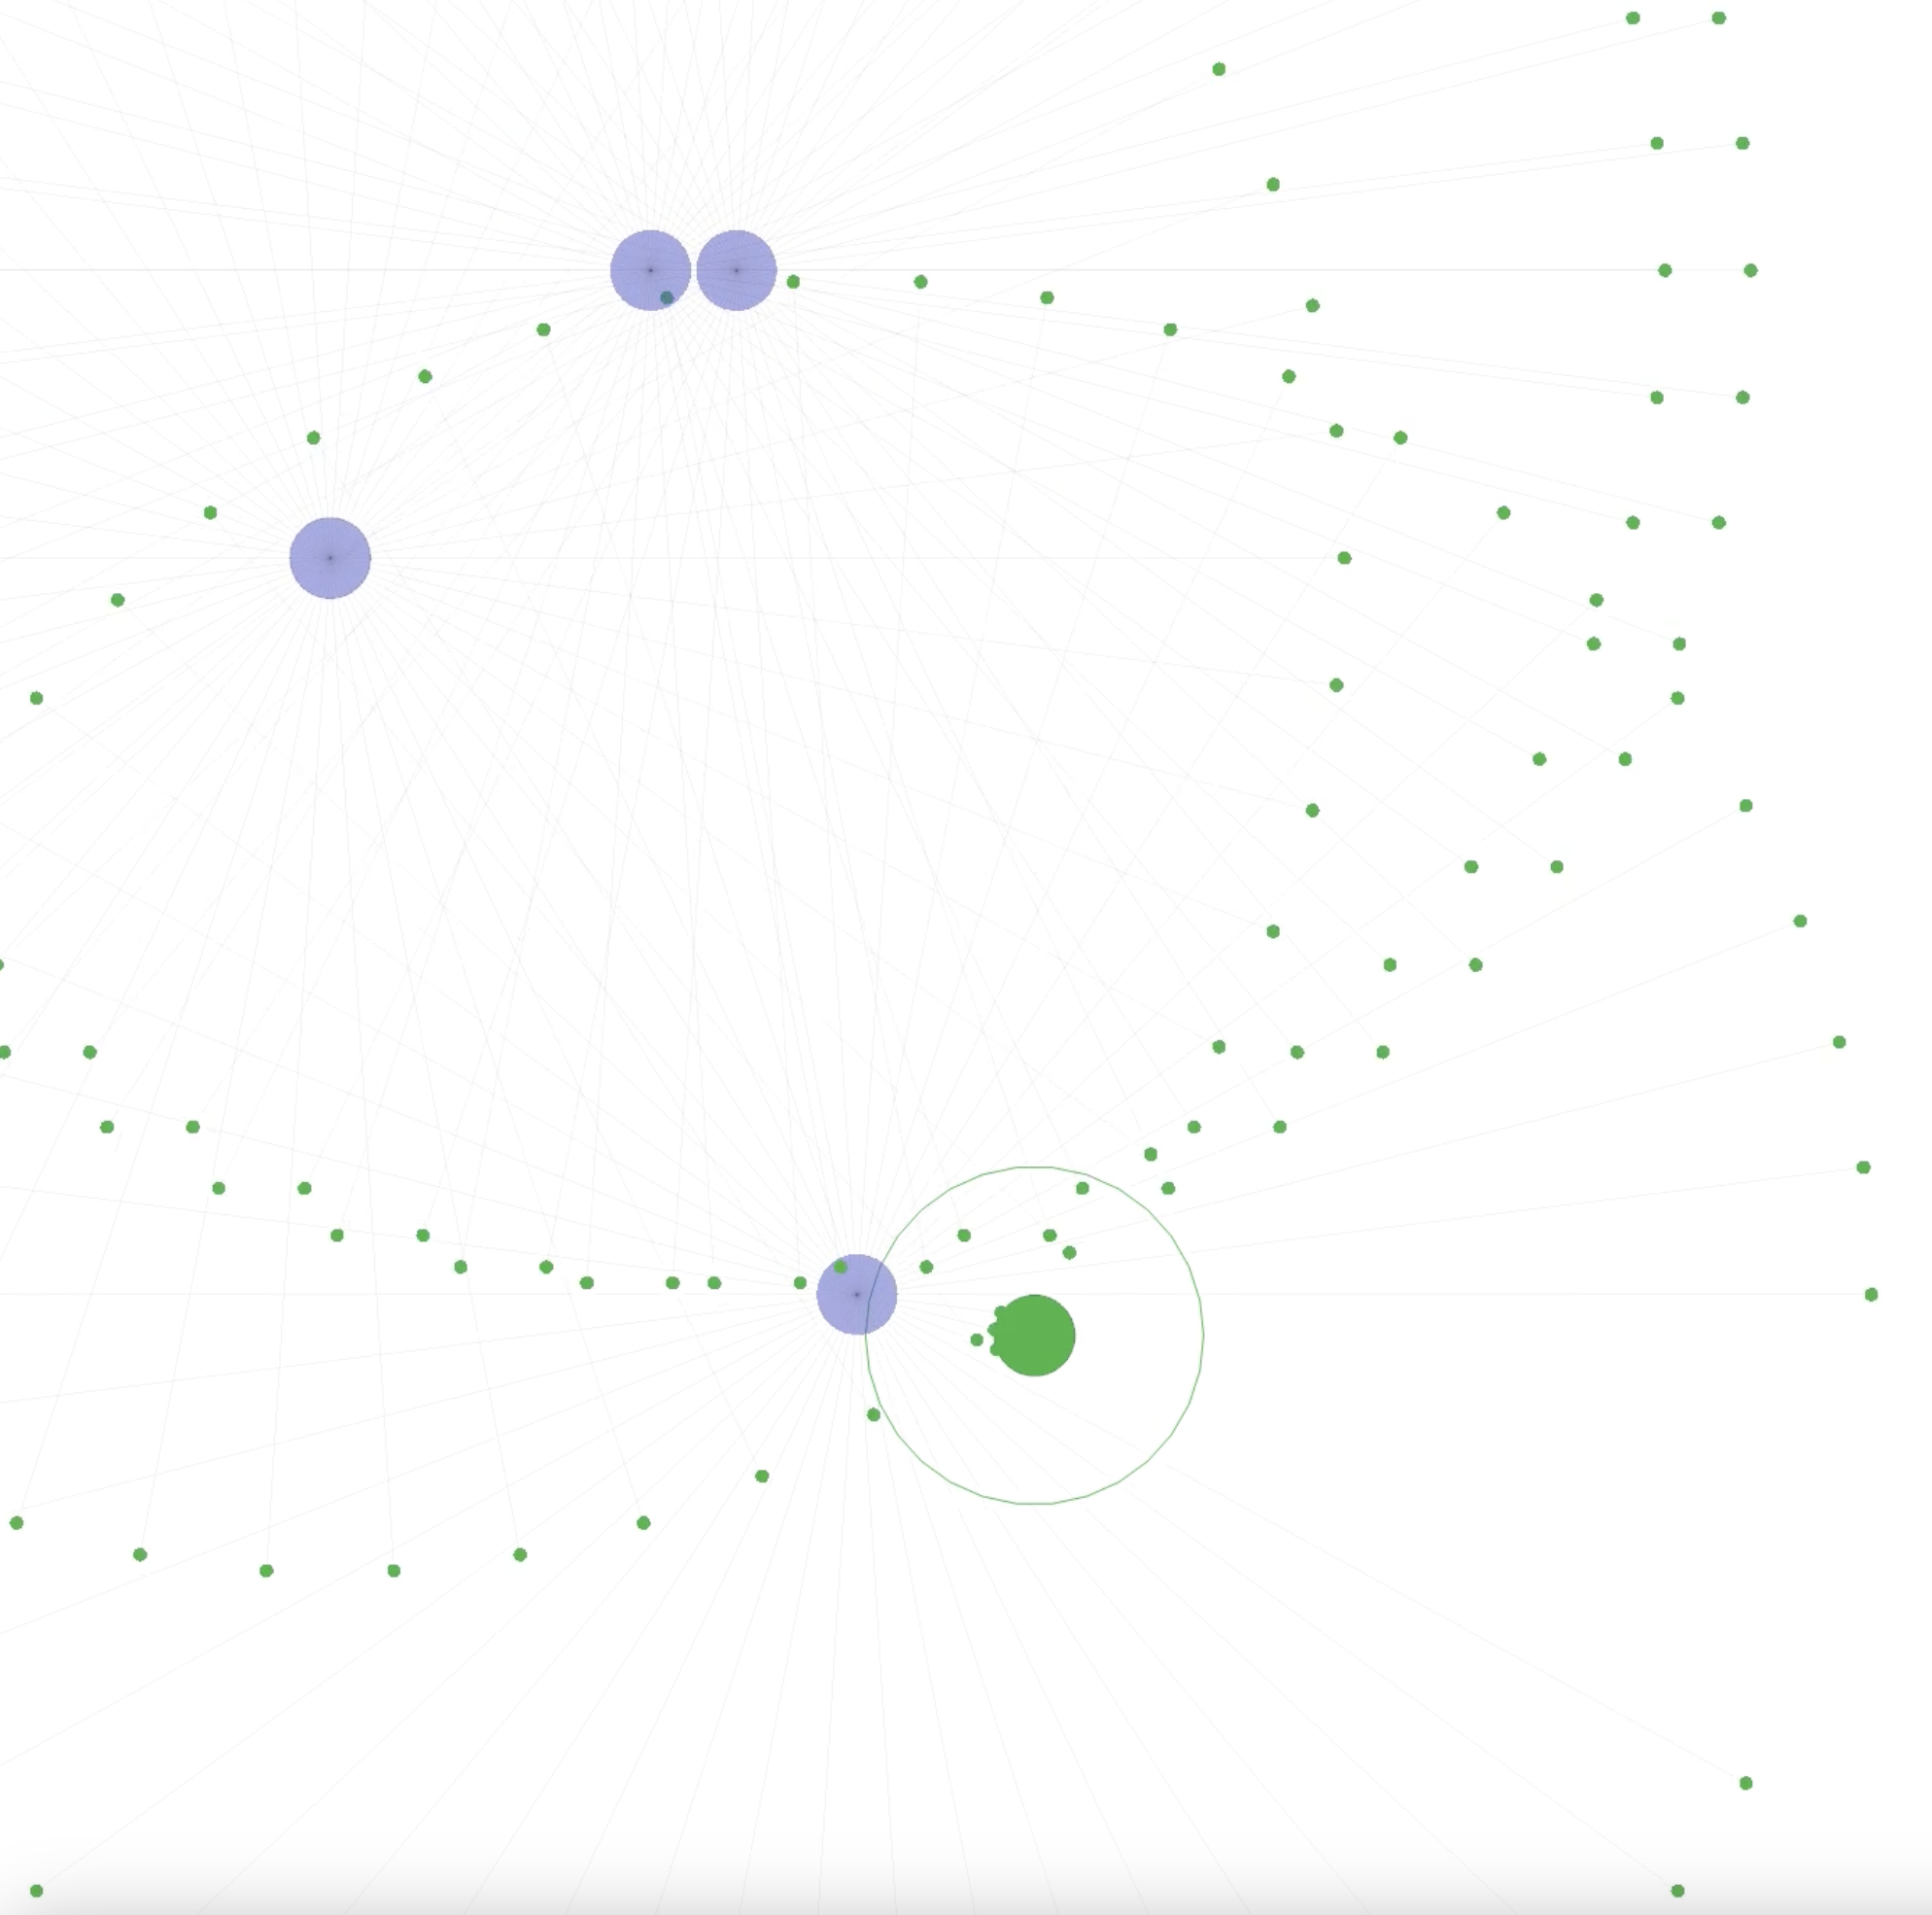
\includegraphics[width=\textwidth]{img/4_agents_3.png}
      \caption{End of simulation} 
  \end{subfigure}
  \caption{Different stages of a simulation with four agent and 14 targets}
  \label{fig:n}
\end{figure}

In a more challenging scenario with four agents and fourteen targets [\ref{fig:n}], the outcomes were as follows:
\begin{itemize}
  \item Agents demonstrated improved collaboration, taking an average of about 400 steps to clear all fourteen targets.
  \item The first target was removed in an average of 10 steps, emphasizing swift task initiation.
  \item Removal of half the targets was achieved in approximately 240 steps, showcasing efficient teamwork among agents.
\end{itemize}

\begin{figure}
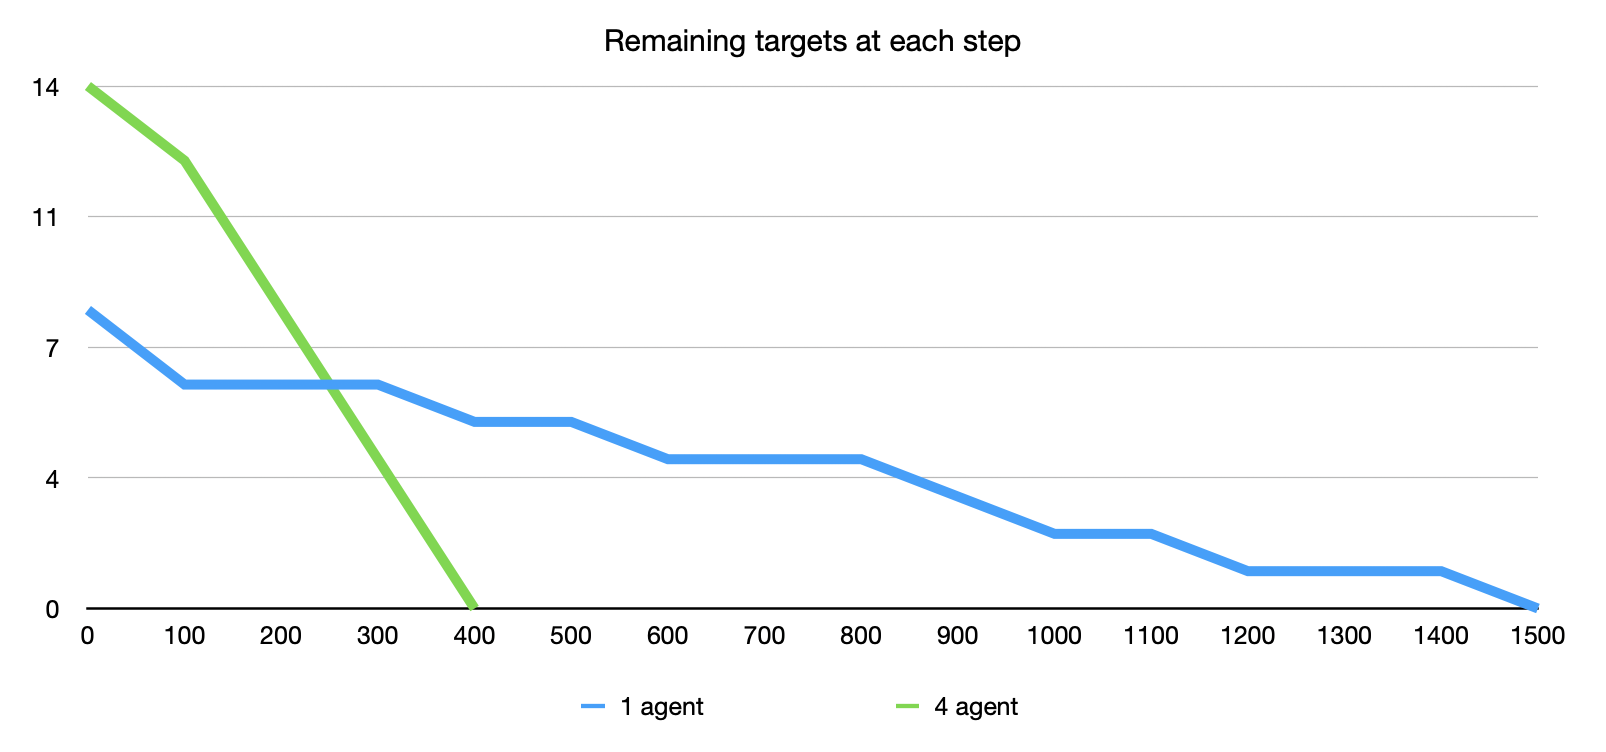
\includegraphics[width=\textwidth]{img/active-targets-per-step.png}
\caption{Remaining targets at each step}
\label{fig:o}
\end{figure}

These performance results underscore the adaptability and learning capabilities of my MLP network-based agents in the Cleaning Agents scenario. As training progressed, agents demonstrated a substantial improvement in their task execution, achieving efficient target removal even in scenarios with multiple agents and numerous targets [\ref{fig:o}].
These findings reflect the effectiveness of my reinforcement learning approach in addressing complex multi-agent coordination tasks.

\subsection{Performance Results: LSTM RNN Networks in the Cleaning Agents Scenario}

The evaluation of LSTM Recurrent Neural Network (RNN)-based agents in the Cleaning Agents scenario provided valuable insights into their learning dynamics and performance. In this scenario, where the environment is partially observable and non-Markovian, the use of LSTM RNNs becomes particularly relevant, as they can capture temporal dependencies and history in a way that traditional feedforward networks cannot.

Employing the same training configuration of 150 epochs, each consisting of 1000 steps, as with the MLP networks, I conducted a rigorous assessment of the LSTM RNN agents. This approach was motivated by prior research \cite{4421430}\cite{4655239}\cite{Banchi_2018} that demonstrated the effectiveness of RNNs in handling non-Markovian environments.

\subsubsection{Training Challenges}

One distinctive characteristic that emerged during the training of LSTM RNN agents was the instability of the loss function throughout the entire training process. Unlike the MLP networks, where the loss gradually stabilized, the LSTM RNN exhibited a highly erratic loss profile. This instability was indicative of the challenges faced by the agents in learning a coherent policy in a non-Markovian environment. Prior studies (cite relevant research) have acknowledged similar difficulties in training RNNs for tasks with temporal dependencies.

Additionally, the performances of the agents appeared to be highly random, with outcomes seemingly influenced by previous actions, even when those actions resulted in extremely negative rewards. This behavior underscores the need for more advanced modeling techniques to capture the complex temporal relationships in the Cleaning Agents scenario.

\subsubsection{Evaluation Uncertainty}

The evaluation phase of LSTM RNN agents presented significant challenges as well. The results obtained during evaluation were notably unreliable and inconsistent. It became apparent that the agents' performances were largely unpredictable, often influenced by casual factors rather than the effectiveness of the model itself. Even after multiple attempts and evaluations, the LSTM RNN-based agents consistently struggled to achieve the desired task of removing all targets within the Cleaning Agents scenario.

This unpredictability further highlights the non-Markovian nature of the scenario, where past actions and states play a significant role in shaping future behavior.

\subsubsection{Ongoing Difficulties}

Despite numerous iterations and training efforts, the LSTM RNN agents faced persistent difficulties in mastering the Cleaning Agents scenario. The model's inherent complexity and the recurrent nature of the networks seemed to introduce challenges in learning a stable and effective policy for tasks with non-Markovian dependencies. The highly variable and unpredictable outcomes during evaluation indicated a significant gap in performance compared to the MLP network-based agents.

In conclusion, the use of LSTM RNN-based agents in the Cleaning Agents scenario, which features a partially observable and non-Markovian environment, encountered substantial challenges in training and evaluation. The instability of the loss function, coupled with erratic agent performances, raised concerns about the suitability of this architecture for the task. Despite repeated attempts, the agents were unable to consistently achieve the goal of removing all targets, highlighting the need for further investigation and potentially alternative approaches in addressing the complexities of multi-agent coordination tasks in this scenario.

\newpage

\addcontentsline{toc}{section}{Bibliography}
%\bibliographystyle{unsrt}
%\bibliography{bibliografia}
\printbibliography %Prints bibliography


\end{document}
